%%
% The BIThesis Template for Bachelor Graduation Thesis
%
% 北京理工大学毕业设计(论文) —— 使用 XeLaTeX 编译
%
% Copyright 2021-2023 BITNP
%
% This work may be distributed and/or modified under the
% conditions of the LaTeX Project Public License, either version 1.3
% of this license or (at your option) any later version.
% The latest version of this license is in
%   http://www.latex-project.org/lppl.txt
% and version 1.3 or later is part of all distributions of LaTeX
% version 2005/12/01 or later.
%
% This work has the LPPL maintenance status `maintained'.
%
% The Current Maintainer of this work is Feng Kaiyu.
%
% Compile with: xelatex -> biber -> xelatex -> xelatex

% !TeX program = xelatex
% !BIB program = biber


% 开启盲审格式 blindPeerReview=true (如:[type=bachelor,blindPeerReview=true])

\documentclass[type=bachelor]{bithesis}

\BITSetup{
  cover = {
    % 在封面中载入有「北京理工大学」字样的图片,如无必要请勿改动。
    headerImage = images/header.png,
    % 在封面标题中使用思源黑体,使用此选项可以保证与 Word 封面标题的字体一致。
    xiheiFont = STXIHEI.TTF,
    %% 使用以下参数来自定义封面日期
    % date = 2022年6月,
  },
  info = {
    % 想要删除某项封面信息,直接删除该项即可。
    % 想要让某项封面信息留空(但是保留下划线),请设置为空字符串。
    % 如需要换行,则用 “\\” 符号分割。
    title = 树状区块链测试与改进,
    titleEn = {The Testing and Enhancements of Tree-Like Blockchain},
    school = 计算机学院,
    major = 计算机科学与技术,
    class = 07111905,
    author = 傅泽,
    studentId = 1120192062,
    supervisor = 陆慧梅,
    keywords = {北京理工大学;本科生;毕业设计(论文)},
    keywordsEn = {BIT; Undergraduate; Graduation Project (Thesis)},
    % 如果你的毕设为校外毕设,请将下面这一行语句解除注释(删除第一个百分号字符)并填写你的校外毕设导师名字
    % externalSupervisor = 左偏树,
  },
  style = {
    % 保持参考文献的缩进样式与 Word 模板一致。
    % 如果你不需要此样式,请将此行注释掉。
    bibliographyIndent = false,
  }
}

% 使用 listings 宏包进行代码块使用,并使用了预定义的样式,
% 你也可以选用自己的喜欢的其他宏包,如 minted;
% 然而由于 minted 依赖 Python 的 Pygments 库作为外部依赖,因此出于模板的简洁程度考虑,我们没有提供 minted 进行代码块书写的示例。
\usepackage{listings}
\definecolor{Orange}{RGB}{255,127,39}

\lstset{
  basicstyle          =   \ttfamily,          % 基本代码风格
  keywordstyle        =   \bfseries\color{Orange}, % 设置关键字为粗体,颜色为 NavyBlue
  commentstyle        =   \rmfamily\itshape,  % 注释的风格,斜体
  stringstyle         =   \ttfamily,  % 字符串风格
  flexiblecolumns,                % 别问为什么,加上这个
  numbers             =   left,   % 行号的位置在左边
  showspaces          =   false,  % 是否显示空格,显示了有点乱,所以不现实了
  numberstyle         =   \zihao{-5}\ttfamily,    % 行号的样式,小五号,tt等宽字体
  showstringspaces    =   false,
  captionpos          =   t,      % 这段代码的名字所呈现的位置,t指的是top上面
  frame               =   lrtb,   % 显示边框
  breaklines = true,
}

\usepackage[
  backend=biber,
  style=gb7714-2015,
  gbalign=gb7714-2015,
  gbnamefmt=lowercase,
  gbpub=false,
  doi=false,
  url=false,
  eprint=false,
  isbn=false,
]{biblatex}

% 参考文献引用文件位于 misc/ref.bib
\addbibresource{misc/ref.bib}


% 文档开始
\begin{document}

% 标题页面:如无特殊需要,本部分无需改动
% \input{misc/0_cover.tex}
\MakeCover

% 原创性声明:如无特殊需要,本部分无需改动
% 更改为 PDF 页面插入,如需要添加内容,可考虑先用 Word 制作再覆盖 misc/1_originality.pdf
% ====== 原创性声明(PDF 格式)======
\begin{blindPeerReview}
  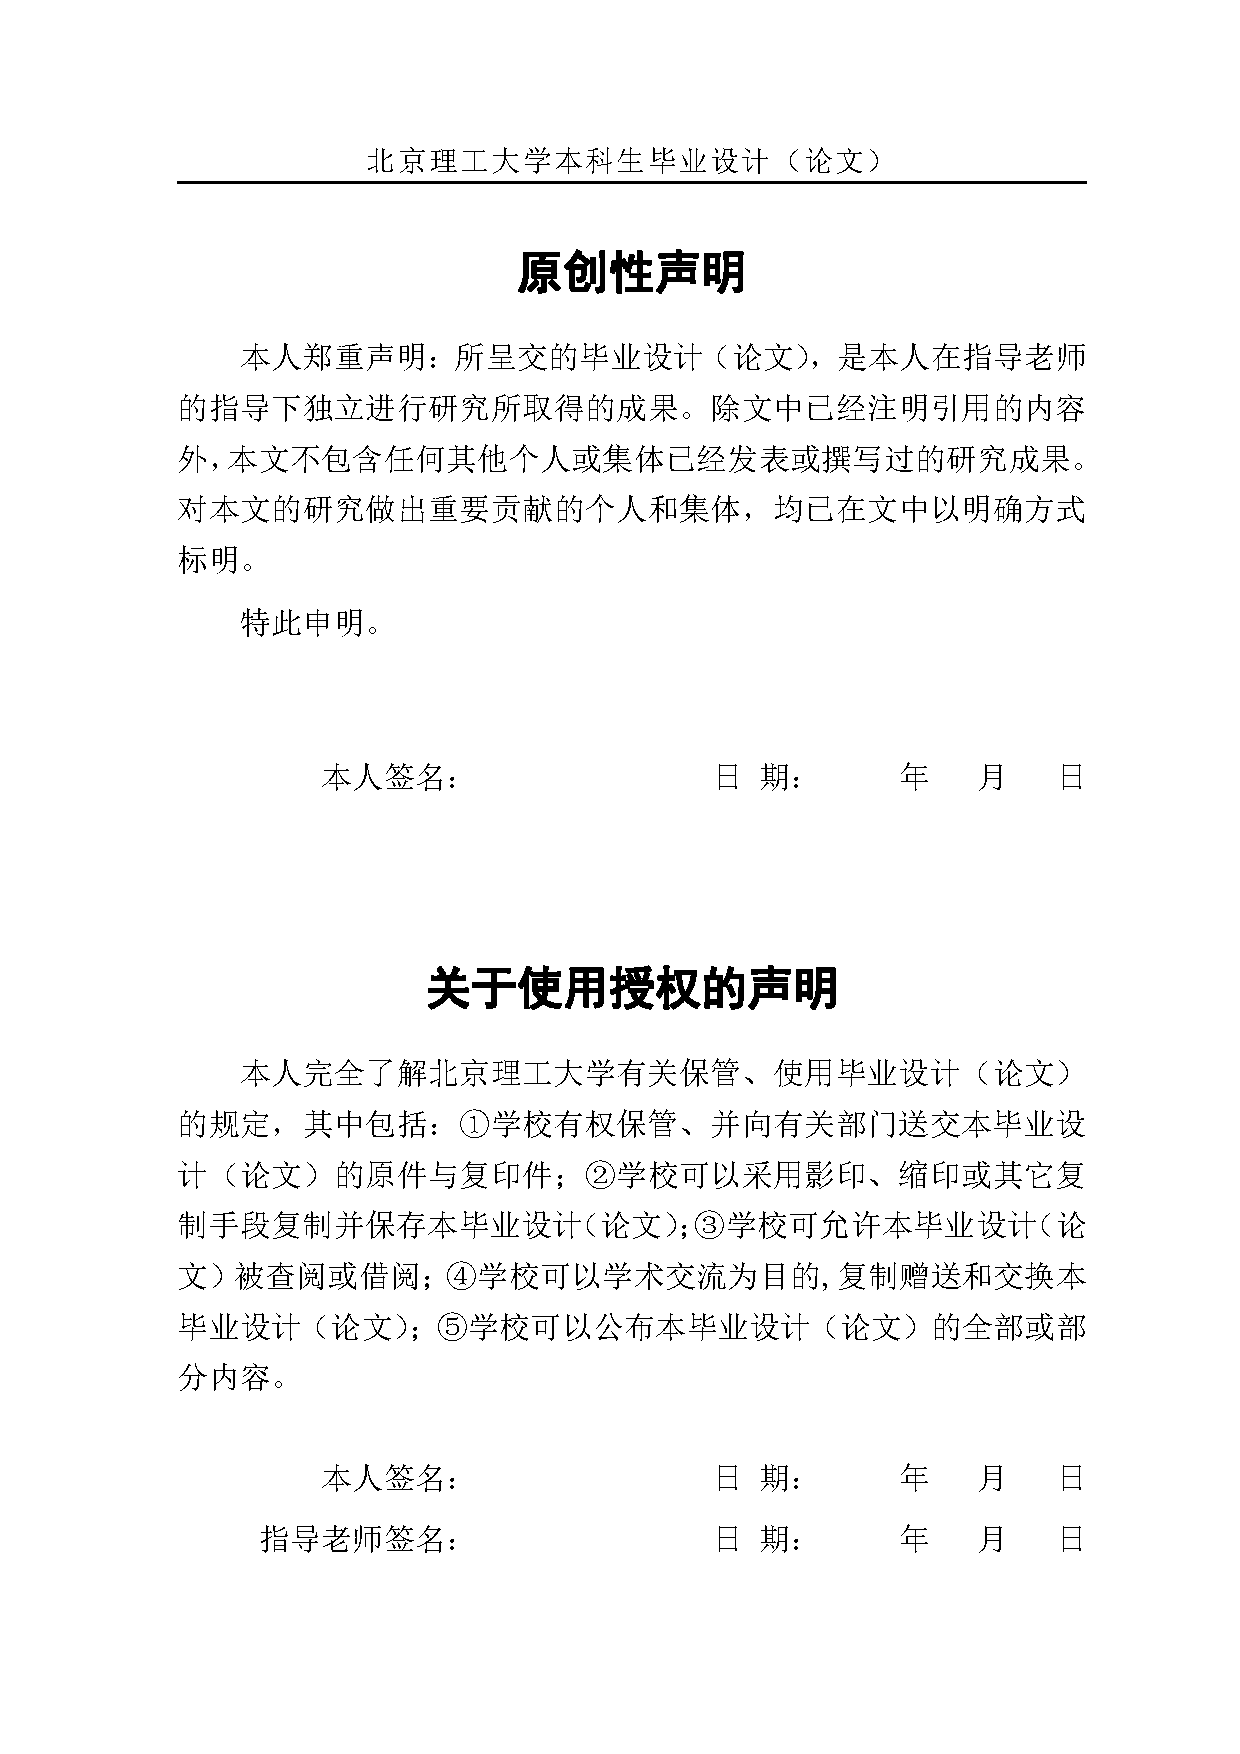
\includepdf{misc/1_originality.pdf}\newpage
\end{blindPeerReview}
% ====== 原创性声明(PDF 格式)======
% ====== 原创性声明(LaTeX 格式)======
% %%
% The BIThesis Template for Bachelor Graduation Thesis
%
% 北京理工大学毕业设计(论文)原创性声明模板 —— 使用 XeLaTeX 编译
%
% Copyright 2020-2022 BITNP
%
% This work may be distributed and/or modified under the
% conditions of the LaTeX Project Public License, either version 1.3
% of this license or (at your option) any later version.
% The latest version of this license is in
%   http://www.latex-project.org/lppl.txt
% and version 1.3 or later is part of all distributions of LaTeX
% version 2005/12/01 or later.
%
% This work has the LPPL maintenance status `maintained'.
%
% The Current Maintainer of this work is Feng Kaiyu.
%
% Compile with: xelatex -> biber -> xelatex -> xelatex
%
% 如无特殊需要,本页面无需更改

\MakeOriginality

% ====== 原创性声明(LaTeX 格式)======

% 前置页面定义
\frontmatter
% 摘要:在摘要相应的 TeX 文件处进行摘要部分的撰写
%%
% The BIThesis Template for Bachelor Paper Translation
%
% 北京理工大学毕业设计(论文) —— 使用 XeLaTeX 编译
%
% Copyright 2020-2023 BITNP
%
% This work may be distributed and/or modified under the
% conditions of the LaTeX Project Public License, either version 1.3
% of this license or (at your option) any later version.
% The latest version of this license is in
%   http://www.latex-project.org/lppl.txt
% and version 1.3 or later is part of all distributions of LaTeX
% version 2005/12/01 or later.
%
% This work has the LPPL maintenance status `maintained'.
%
% The Current Maintainer of this work is Feng Kaiyu.
%
% Compile with: xelatex -> biber -> xelatex -> xelatex
%%

% 中文摘要
\begin{abstract}
% 中文摘要正文从这里开始
本文为笔者的Substrate区块链工具套件官方英文文档的中文翻译。其包含原文的“快速上手”章节的全部内容,以及“基础知识”章节中的“区块链基础”、“为何选择Substrate”、“Substrate是什么”、“架构”和“网络与区块链”部分的内容。

\end{abstract}


\MakeTOC

% 正文开始
\mainmatter

% 第一章
%%
% The BIThesis Template for Bachelor Graduation Thesis
%
% 北京理工大学毕业设计(论文)第一章节 —— 使用 XeLaTeX 编译
%
% Copyright 2020-2023 BITNP
%
% This work may be distributed and/or modified under the
% conditions of the LaTeX Project Public License, either version 1.3
% of this license or (at your option) any later version.
% The latest version of this license is in
%   http://www.latex-project.org/lppl.txt
% and version 1.3 or later is part of all distributions of LaTeX
% version 2005/12/01 or later.
%
% This work has the LPPL maintenance status `maintained'.
%
% The Current Maintainer of this work is Feng Kaiyu.
%
% 第一章节

\chapter{绪论}

\section{研究背景}

区块链是一种分布式的共享账本,允许数个参与方一同共享数据。区块链技术所拥有的去中心化、透明性和安全性等优势,令这一新兴的概念迅速为各行各业接受:中国人民银行数字货币研究所正在积极探索区块链技术在低并发、低敏感的资产确权、交易转让、账本核对等场景下的应用\cite{shuYanSuo};区块链透明化的特点和极高的安全性也引起了地产行业的注意\cite{usageOfBC}。可以预见,区块链技术在未来将吸引更多行业加入,以其去中心化、不可篡改等特性造福人类社会。

树状区块链,是实验室正在开发并已趋于完善的改良型区块链。其基本思想大致为:将区块分为创世块、分支区块和叶子区块三种;结合GeoHash编码技术,不再采用传统区块链的单链结构,形成类似于字典树的树状结构;同时,为了满足快速查询的需要,在区块中增添了一些辅助数据结构。经过以上改良,树状区块链可以在对地理位置敏感、且网络结构变化较频繁的应用场景中,发挥相较传统区块链更好的理论性能。

车联网技术(Internet of Vehicle)属于物联网技术的范畴,其思想乃是在车辆上搭载接入网络的设备,旨在实现不同车辆之间的相互通信;不仅如此,车联网技术也容许车辆与行人、路边基站等交通参与方和交通基础设施通信,实现实时的车况检测、路况查询与收集等功能,对于提升车主用车体验、乘客出行体验有强大的潜力。2022年12月8日,公安部发布的数据显示全国机动车保有量到达4.15亿辆,机动车驾驶员人数超过5亿位!随着如何安全有效地管理如此庞大的保有量带来的海量数据这一巨大挑战变得日益严峻,人们纷纷将目光转移到了区块链上\cite{bcInIoV}。然而,传统区块链在处理车联网场景下的具体事务时,往往存在诸如此类的一些弊端:

\begin{itemize}
  \item 车辆作为区块链网络的参与者(节点)时,其地理位置可能发生很大变化,致使网络结构需要频繁更新;
  \item 传统区块链采用单链结构,在区块链上执行的查询时间复杂度较高;
  \item 在车联网系统中,车辆应该关心的信息大部分来自于其所在位置的临近街区,而传统区块链并不以地理位置索引区块及其交易,故一次查询可能会获得较多无用信息等。
\end{itemize}

由于树状结构相比单链结构的深度更小,且采用了与地理位置相关的GeoHash进行分支构造,故有效降低了查询开销,令基于位置的信息查询能够更加“有的放矢”,有望为运用区块链技术处理车联网问题提供合理可行的解决方案。

目前,实验室已有的树状区块链采用以太坊(Ethereum)实现。以太坊是一个开源的区块链计算平台,允许开发者进行去中心化应用程序(DApp)的开发和部署。其支持以Solidity编程语言编写运行在在以太坊虚拟机上的脚本程序(智能合约Smart Contract),极大拓宽了区块链的功能适用性。

Substrate是一组开源、模块化的区块链开发框架,允许开发者自由地使用官方预定义的各种组件构建个性化的区块链,并于其上使用基于Rust的ink!编程语言进行智能合约开发。与以太坊比较,Substrate具有包括而不仅限于如下优势:

\begin{itemize}
  \item 支持模块化设计,程序员可以轻松增删模块,构建更加贴近实际需求的区块链
  \item 采用Rust编程语言作为其底层实现,速度更快,效率更高
  \item 支持编译为大多数现代浏览器支持的WebAssembly二进制,提供了更好的跨平台兼容性
\end{itemize}

本文将在车联网的应用场景下,以实验室已有工作——出租车调度系统为例,探究树状区块链在不同工况下的性能表现,验证其拥有相较传统单链区块链更好的性能表现。本文还将积极尝试为将树状区块链从以太坊平台转向更优秀的Substrate平台。鉴于时间和笔者能力之限,本文仅讨论从上层应用系统——出租车调度系统的智能合约部分的迁移工作,此举旨在验证两平台在功能上的相似性,进而确保未来树状区块链的底层功能迁移工作的可行性。

\section{相关技术调研}

\subsection{区块链技术概述}

2008年,一位自称为中本聪的人发布了名为《Bitcoin: A Peer-to-Peer Electronic Cash System》的论文,宣告了区块链技术的诞生。区块链,乃是一个分布式的账本;区块链网络不存在所谓的“中心服务器”,每台参与构成区块链网络的计算机(又被称为“节点”)均持有一份该账本的副本。每一笔交易,都将记录在名为“区块”的数据结构中;随着区块的不断产生,它们将形成一条单向链状结构,且区块上存储的数据将不可再被修改。通过称为共识算法的机制,各节点能够就区块链的当前状态达成一致,并在链上数据发生变化时及时追踪并更新到自身存储的账本中。不仅如此,若某个节点尝试擅自修改自身所持有的账本,其行为会被共识算法拒绝,从而规避了恶意篡改链上数据的风险。上述区块链的优势,令区块链这一新兴的概念迅速吸引了各行各业的眼球。可以预见,区块链技术在未来将吸引更多行业加入,以其去中心化、不可篡改等特性造福人类社会。

\subsection{智能合约概述}

智能合约(Smart Contract)这一概念由Nick Szabo于1994年提出。在比特币的支付模型中,仅存在一个简单的堆栈计算机。由于其可用的操作方法并非图灵完备,只能执行比较简单的操作,从而限制了区块链的应用场景。智能合约的出现打破了这一局面。在Szabo于1996年撰写的《Smart Contracts: Building Blocks for Digital Markets》一文\cite{nickSzabo}中,Nick设想智能合约就是运行在区块链上的一段程序,当满足某种条件时,相应代码将自动被执行,而该过程人类无需也无法介入。智能合约一定程度上避免了交易双方抵赖的问题,并且其图灵完备的特性也令区块链技术在不同应用场景下的适应性大大增加了。

\subsection{区域索引区块链和树状区块链概述}

周畅设计的区域索引区块链,实现了区块链地理信息索引方法,能够依据地理位置信息快速查询特定位置的交易\cite{sensors}。如图1-1所示,相较以太坊官方实现的传统区块链而言,区域索引区块链在区块头中加入了区域状态树的树根哈希,以支持基于位置的快速信息查询;同时,为追踪每个账户的包括位置信息的完整状态,在账户状态数据结构中还加入了当前的地理位置字段、和账户位置树这一数据结构。不仅如此,在记录交易、收据时,均会记录发起动作的地理位置信息,并以此更新发起人的账户的当前位置及账户位置树。文献\cite{sensors}中指出,采用3到6位GeoHash编码时,区域索引区块链相较传统的无索引区块链,执行相同查询的耗时仅为后者的5.3\%。

\begin{figure}[htbp]
  \centering
  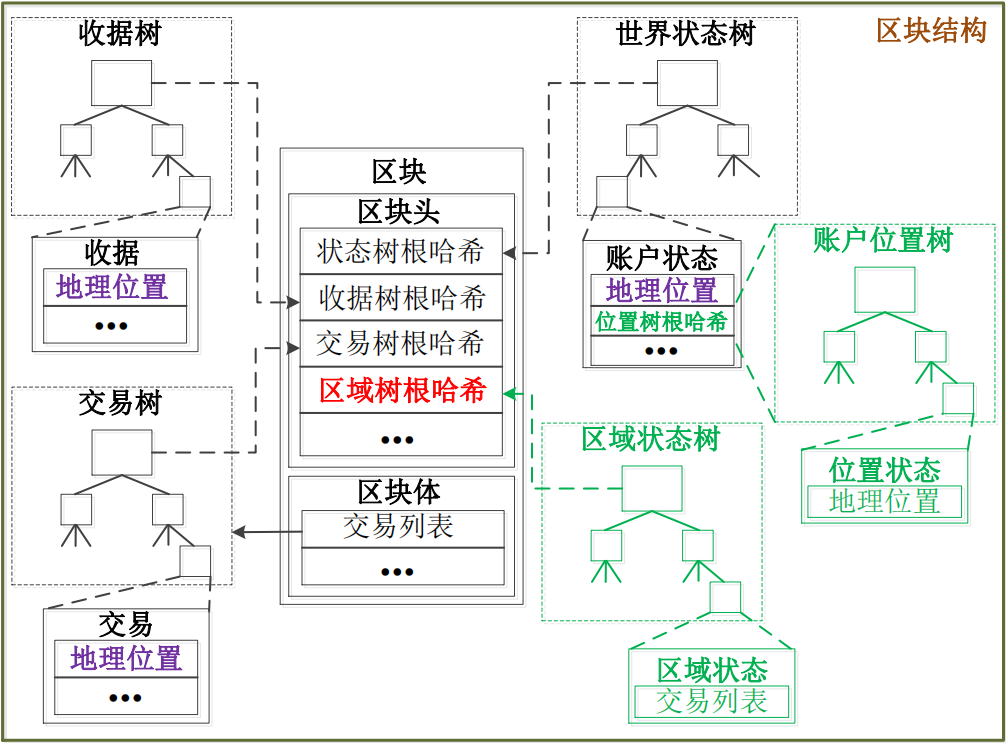
\includegraphics[width=0.7\textwidth]{images/区域链区块示意图.png}
  \caption{区域链区块示意图}\label{区域链区块示意图} % label 用来在文中索引
\end{figure}

区域索引区块链仍然保留了传统区块链的单链结构,当区块数量很大时,其查询效率仍然会随之降低。因此,周畅提出并设计了基于区域索引区块链改良的树状区域索引区块链(下简称树状区块链)。其按照Geohash编码长度,表示父链和子链的关系,并划分区域子链。树状区块链的区块也分为三种:叶子区块、分支区块和创世块。叶子区块和传统的区块链并无太大差异,叶子区块及其后续区块均采用传统的单链结构加以组织;分支区块则负责将数个叶子区块组织起来,按照叶子区块所代表的地理位置,创世块和分支区块十分相似,但它没有父链指针。上述树状区块链的设计,进一步缩短了区块链网络中的单链长度,进而提升了查询效率。

\subsection{以太坊虚拟机和WebAssembly}
% 顺手介绍一下以太坊和Substrate

\section{本文研究内容及贡献}

本文将在车联网这一应用场景下,首先基于区域索引区块链,复现实验室已有工作——出租车调度系统的有关工作,证明该系统的可用性。此后,设计并进行树状区域索引区块链在单父链双子链的网络结构下的跨链转账实验,探究树状区块链在不同转账请求压力下的性能表现,验证其功能可用性,并测试跨链操作带来的额外时间开销。作为测试实验的收尾,本文将设计实验,令出租车调度系统分别在网络结构不同的树状区块链上运行,收集并可视化实验数据,评估树状区块链在不同工况的实际应用场景下的性能表现。本文还将为树状区块链从以太坊平台转向更优秀的Substrate平台做出积极探索。鉴于时间和笔者能力之限,本文仅讨论从上层应用系统——出租车调度系统的智能合约部分的迁移工作,此举旨在验证两平台在功能上相似,进而证明未来树状区块链的底层功能迁移工作的可行性。

\begin{enumerate}
  \item 基于区域索引区块链,复现实验室已有工作——出租车调度系统,证明该系统的可用性;编写帮助文档和实验日志,以便后人推进研究
  \item 设计并进行树状区域索引区块链在单父链双子链的网络结构下的跨链转账实验,记录其对10个、20个、40个、80个、120个、160个、200个账号执行子链之间的跨链转账的耗时、吞吐量等数据,并进行可视化;编写帮助文档和实验日志,以便后人推进研究
  \item 在单子链、单父链四子链的网络结构下分别运行出租车调度系统,探究树状区块链在不同工况实际场景中的性能表现,并进行数据可视化;编写帮助文档和实验日志,以便后人推进研究
  \item 探索上层应用系统从以太坊向Substrate的迁移,将出租车调度系统的部分智能合约从Solidity语言重新编写为ink!语言,并进行单元测试,确保在重新编写前后合约的语义一致;编写实验日志,以便纠错和改进
\end{enumerate}

\section{二级题目}
% 这里插入一个参考文献,仅作参考

\subsection{三级题目}

正文……\cite{yuFeiJiZongTiDuoXueKeSheJiYouHuaDeXianZhuangYuFaZhanFangXiang2008}……\cite{Hajela2012Application}

\textcolor{blue}{正文部分:宋体、小四;正文行距:22磅;间距段前段后均为0行。阅后删除此段。}

\textcolor{blue}{图、表居中,图注标在图下方,表头标在表上方,宋体、五号、居中,1.25倍行距,间距段前段后均为0行,图表与上下文之间各空一行。阅后删除此段。}

\textcolor{blue}{\underline{\underline{图-示例:(阅后删除此段)}}}


\begin{figure}[htbp]
  \centering
  
\includegraphics[]{images/bit_logo.png}
  \caption{标题序号}\label{标题序号} % label 用来在文中索引
\end{figure}

\textcolor{blue}{\underline{\underline{表-示例:(阅后删除此段)}}}
% 三线表
\begin{table}[htbp]
  \linespread{1.5}
  \zihao{5}
  \centering
  \caption{统计表}\label{统计表}
  \begin{tabular}{*{5}{>{\centering\arraybackslash}p{2cm}}} \toprule
    项目    & 产量    & 销量    & 产值   & 比重    \\ \hline
    手机    & 1000  & 10000 & 500  & 50\%  \\
    计算机   & 5500  & 5000  & 220  & 22\%  \\
    笔记本电脑 & 1100  & 1000  & 280  & 28\%  \\
    合计    & 17600 & 16000 & 1000 & 100\% \\ \bottomrule
  \end{tabular}
\end{table}

\textcolor{blue}{公式标注应于该公式所在行的最右侧。对于较长的公式只可在符号处(+、-、*、/、$\leqslant$ $\geqslant$ 等)转行。在文中引用公式时,在标号前加“式”,如式(1-2)。阅后删除此
  段。}

\textcolor{blue}{公式-示例:(阅后删除此段)}
% 公式上下不要空行,置于同一个段落下即可,否则上下距离会出现高度不一致的问题
\begin{equation}
  LRI=1\ ∕\ \sqrt{1+{\left(\frac{{\mu }_{R}}{{\mu }_{s}}\right)}^{2}{\left(\frac{{\delta }_{R}}{{\delta }_{s}}\right)}^{2}}
\end{equation}

\subsubsection{生僻字}

% 一个可能无法正常显示的生僻字
% 一个可能无法正常显示的生僻字: 彧。下文注释中,介绍了如何通过自定义字体来显示生僻字。

% 定义一个提供了生僻字的字体,注意要确保你的系统存在该字体
% \setCJKfamilyfont{custom-font}{Noto Serif CJK SC}

% 使用自己定义的字体
% 使用提供了相应字型的字体:\CJKfamily{custom-font}{彧}。


% 在这里添加第二章、第三章……TeX 文件的引用
%%
% The BIThesis Template for Bachelor Graduation Thesis
%
% 北京理工大学毕业设计(论文)第二章节 —— 使用 XeLaTeX 编译
%
% Copyright 2020-2023 BITNP
%
% This work may be distributed and/or modified under the
% conditions of the LaTeX Project Public License, either version 1.3
% of this license or (at your option) any later version.
% The latest version of this license is in
%   http://www.latex-project.org/lppl.txt
% and version 1.3 or later is part of all distributions of LaTeX
% version 2005/12/01 or later.
%
% This work has the LPPL maintenance status `maintained'.
%
% The Current Maintainer of this work is Feng Kaiyu.
%%

\chapter{基于区域索引区块链的出租车调度系统复现}

本章讨论基于区域索引区块链的出租车调度系统的复现工作。

基于区域索引区块链的出租车调度系统,以董斌的区块链地图存储作为基础,由成佳壮首先提出并实现路径规划和司乘匹配等算法,并随后经过万琦玲完善,并初步形成了复现手册;它是一套采用实验室已有成果——区域索引区块链作为服务器后端、Vue 2.JS作为前端的出租车调度系统。在万琦玲设计的前端页面上,用户可以通过实时地图信息,直观地获得自己的位置,以及附近在线的乘客、司机等信息。用户角色分为乘客和司机两大类,前者可以进行提交乘车请求、确认上车和付款等操作,而后者可以选择是否接受派来的订单,确认到达乘客上车地点和确认到达乘客下车地点等操作。

本文将基于上述实验室已有工作,进行该基于区域索引区块链的出租车调度系统的复现工作,并详细讲解在复现过程中遇到的问题,及其解决方案。此外,该部分工作还补充了初版复现手册的缺漏,修正了其中的错误,重构了已有的脚本代码,提升了可扩展性和鲁棒性,形成了新版的复现手册,方便后人参考\footnote{https://github.com/Endericedragon/ReproducingBlockchain}。

\section{环境配置}

本文复现工作将在如下环境中进行:

\begin{table}[htbp]
    \linespread{1.5}
    \zihao{5}
    \centering
    \caption{复现环境}\label{复现环境}
    \begin{tabular}{*{5}{>{\centering\arraybackslash}p{6cm}}} \toprule
        中央处理器 & Intel Core i5-12500H      \\
        图形处理器 & Intel Iris Xe 80EU        \\
        内存    & 24GB                      \\
        操作系统  & Ubuntu 22.04.1 LTS        \\
        虚拟机   & VMWare Workstation Pro 17 \\
        \bottomrule
    \end{tabular}
\end{table}

将Ubuntu虚拟机环境配置妥当之后,还需安装node.js、npm、web3.js等JavaScript库。同时,将区域索引区块链的二进制可执行文件(代码仓库中的geth1二进制可执行文件)存放到/usr/local/bin文件夹下备用。

\section{复现步骤}

详细的复现过程已记录于代码仓库的《8 重做调度系统复现实验.md》文档中,本文将只进行简单介绍。需要指明的是,原复现手册中存在许多前置实验,本文略过了这些前置实验,仅详细介绍最后有关调度系统复现的实验。

\subsection{建立区域索引区块链}

启动终端,切换至创世配置文件genesis.json所在的目录,随后键入如下指令并执行:

\begin{lstlisting}[caption={初始化区块链}, label={lst:初始化区块链}]
geth1 --identity "MyEth" --rpc --rpcaddr 127.0.0.1  --rpcport "8545" --rpccorsdomain "*" --datadir gethdata --port "30303" --nodiscover --rpcapi "eth,net,personal,web3,admin" --networkid 91036 init genesis.json
\end{lstlisting}

对于其中的关键参数选项解释如下:

\begin{itemize}
    \item rpcaddr、rpcport:RPC端口的地址及端口号。外部程序可以使用该端口接入区块链,进而借助JSON-RPC API或者web3.js库和区块链进行交互。
    \item datadir:该选项指定链上数据在本地永久存储的位置。
    \item rpcapi:使用RPC端口与链交互时,仅能使用该选项指定的数个功能。本文将使用eth,net,personal,web3,admin这5个功能模块,它们涵盖了挖矿、发现节点、账号管理等功能,足以满足复现实验要求。
    \item init genesis.json:指定使用名为genesis.json的创世配置文件进行初始化。
\end{itemize}

执行结束后,再执行以下命令,即可启动该区块链:

\begin{lstlisting}[caption={启动区块链}, label={lst:启动区块链}]
geth1 --datadir ./gethdata --networkid 91036 --port 30303 --rpc --rpcaddr 127.0.0.1 --rpcport 8545 --rpcapi 'personal,net,eth,web3,admin' --rpccorsdomain='*' --ws --wsaddr='localhost' --wsport 8546 --wsorigins='*' --wsapi 'personal,net,eth,web3,admin' --nodiscover --allow-insecure-unlock --dev.period 1 --syncmode='full' console
\end{lstlisting}

注意其中的syncmode参数选项,其值为'full'。此时,该区块链将仅使用区域索引方法进行加速,而不会使用任何树状区块链的功能特性。

启动区块链后,终端中将出现JavaScript控制台,可以使用JavaScript编程语言的一个子集和链进行交互\cite{gethJS}。此时可以创建测试账户,充当司机和乘客;并且,每次启动区块链,都需要解锁这些账户,否则将无法进行智能合约部署等工作。本文创建了8个测试账户,分别扮演司乘角色,进行后续的实验。

创建账号后,还需前往创世配置文件中,为创建的账号赋予初始余额。赋予余额后,为强制geth1重新加载创世配置文件,需要手动删除存储链上数据的gethdata目录中的geth目录,并随后重新初始化并启动区块链。此时,geth1将从创世块配置信息中加载账户余额,确保后续实验步骤可以正常开展。至此,区域索引区块链已经建立完成。

\subsection{部署合约}

实验室已有成果——出租车调度系统由两份智能合约构成,其文件名和其功能如下表所示:

\begin{table}[htbp]
    \linespread{1.5}
    \zihao{5}
    \centering
    \caption{智能合约功能概述}\label{智能合约功能概述}
    \begin{tabular}{*{5}{>{\centering\arraybackslash}p{4cm}}} \toprule
        文件名              & 功能                                      \\ \hline
        StoreMap.sol     & 存储详细的地图数据,提供数据查询的结构及A-Star寻路等算法的实现      \\
        StoreTraffic.sol & 司机和乘客的信息管理, 提供司乘位置的改查、基于Geohash的距离计算等服务 \\\bottomrule
    \end{tabular}
\end{table}

将两份合约部署到区块链上,即完成树状区块链的部署工作。首先,使用Remix Desktop编译合约,记录编译结果中的ABI字段并进行进行压缩转义,同时记录bytecode(下称字节码)字段。然后,将二者复制入附录B中的代码模板(其中的标识符Contract和contractInstance可以任意修改),将两份编辑好的模板先后复制入正在运行geth1的JavaScript命令行后并点按回车后,合约部署的请求就已经提交至交易池。开始挖矿并密切观察控制台输出,直至观察到形似以下格式的输出。此即为两份合约各自的合约地址,其顺序与提交合约部署申请的顺序一致:

\begin{verbatim}
    null [object Object]
    Contract mined! Address: 0x23b98f92ceac005e570b6768da377b3abd11012e
    [object Object]
    null [object Object]
    Contract mined! Address: 0xfa6b8f0b92b323c28557faf69da028e33856f6ca
    [object Object]
\end{verbatim}

笔者的部署顺序是:先部署StoreMap,再部署StoreTraffic。因此,地图存储合约的地址即为0x23b98f92ceac005e570b6768da377b3abd11012e,而调度合约地址为0xfa6b8f0b92b323c28557faf69da028e33856f6ca。

\subsection{上传地图数据}

成佳壮完成了上传地图所需的JavaScript脚本。使用时,首先需要前往该脚本源代码(对应代码仓库中的\verb|uploadmap_cjz_3.js|),修改其中关于StoreMap合约地址的字符串变量的值、执行数据提交的账号的公钥地址,以及要上传的地图文件。令区块链开始挖矿后,运行该脚本,将看到终端不断输出信息,直至输出“地图数据上传完成”字样,结束挖矿。此时,所有地图数据就已全部上传到区块链上了。

\subsection{配置前端并进行可用性测试}

出租车调度系统的前端由Vue 2写成,在启动之前尚需一些配置方可正常运行。首先,需要修改\verb|investigation-cjzhuang2020/cjz_underg_2021_09|目录下的一系列文件,各个文件的文件名及其内容如下表所示:

\begin{table}[htbp]
    \linespread{1.5}
    \zihao{5}
    \centering
    \caption{前端配置文件功能}\label{前端配置文件功能}
    \begin{tabular}{*{5}{>{\centering\arraybackslash}p{6cm}}} \toprule
        文件名                  & 功能                                            \\ \hline
        passengerAccounts.py & 存储扮演乘客角色的账号的公钥                                \\
        vehicleAccounts.py   & 存储扮演司机角色的账号的公钥                                \\
        mapContract.js       & 关于地图智能合约的调用,需要修改合约地址,与2.2.2节记录的StoreMap合约地址一致 \\
        trafficContract.js   & 关于路径规划合约的调用,需要修改合约地址,与2.2.2节记录的StoreMap合约地址一致 \\
        passengers.js        & 存储每一位乘客的起始位置、上车位置和目的地位置                       \\
        vehicles.js          & 存储每一位司机的初始位置                                  \\\bottomrule
    \end{tabular}
\end{table}

完成以上配置后,即可在区块链中开始挖矿,启动\verb|vehicle_test.py|,程序将打开浏览器并自动操作,可观察到如下图的字样:

\begin{figure}[htbp]
    \centering
    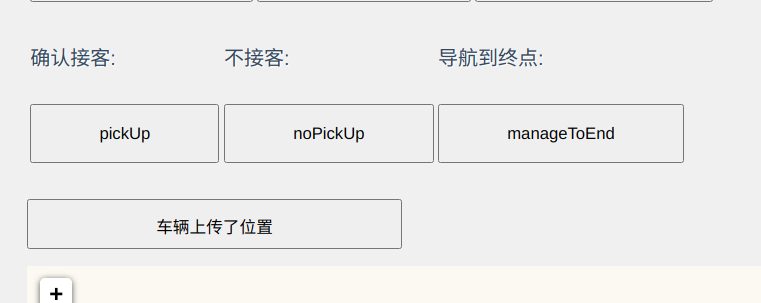
\includegraphics[width=0.8\textwidth]{images/vehicleInit.png}
    \caption{司机的初始化}\label{司机的初始化} % label 用来在文中索引
\end{figure}

此时启动\verb|passenger_test.py|,程序将启动另一个浏览器窗口操作,此时需要在司机端浏览器窗口选择接客与否:

\begin{figure}[htbp]
    \centering
    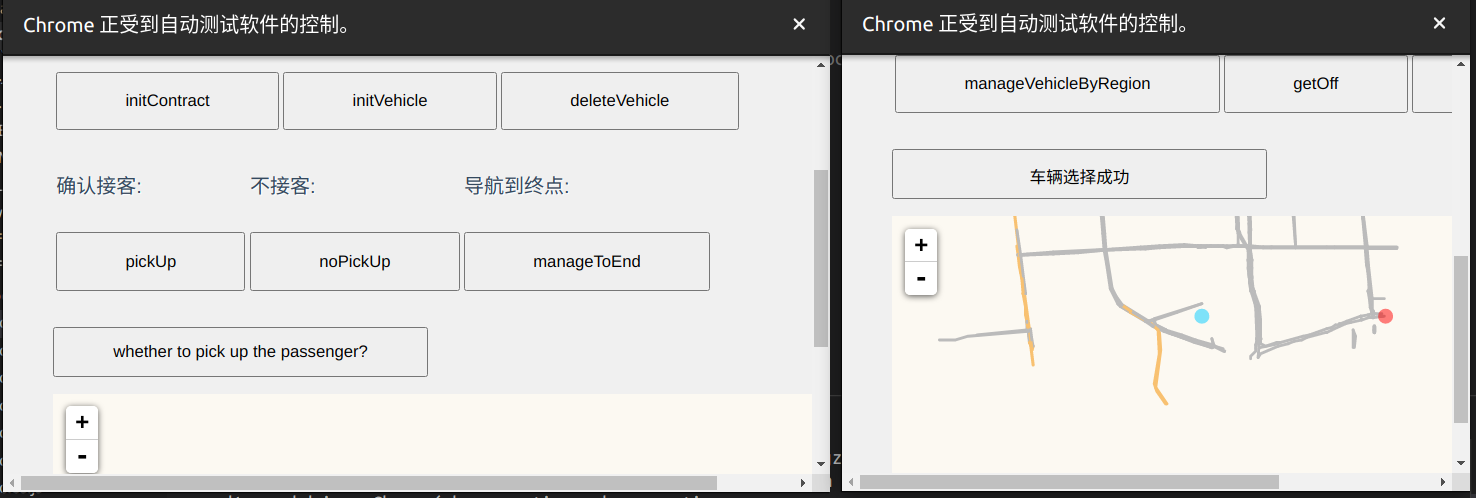
\includegraphics[width=0.8\textwidth]{images/pickUp.png}
    \caption{司机手动接客}\label{司机手动接客} % label 用来在文中索引
\end{figure}

按下pickUp按钮,程序将继续自动运行,直至看到如下输出,调度成功:

\begin{figure}[htbp]
    \centering
    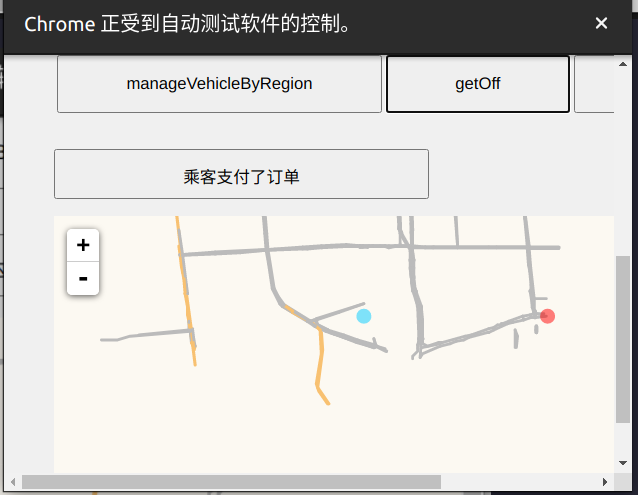
\includegraphics[width=0.8\textwidth]{images/passengerPay.png}
    \caption{乘客抵达并支付}\label{司机手动接乘客抵达并支付客} % label 用来在文中索引
\end{figure}

至此,原复现手册中的所有预期结果均已达到,调度系统复现实验全部完成。

\section{问题及解决方案}

笔者在进行出租车调度系统复现实验及其前置时,遇到许多原复现手册中未提及或未强调的注意事项;原版代码中,亦存在已废弃的语法和有待改进的设计。本节将陈述笔者遇到的问题及其解决方法。

\subsection{创世配置文件指代不明}

原复现手册中,并未指明在进行复现实验时使用的创世配置文件。经过笔者测试,附录A中的创世配置文件可用于所有出租车调度系统复现实验的全部环节。笔者已将其补充到代码仓库和新版复现手册中。

\subsection{节点无法加入区块链网络}

笔者在尝试建立双节点区块链网络时发现,无论如何使用\verb|admin.addPeer()|函数,尝试将第二个节点连接到第一个节点,都无法成功,观察\verb|net.peerCount|的值始终为0,代表着第二个节点并未发现第一个节点。

实际上,节点与区块链网络中的其他节点使用的创世配置文件完全相同,是该节点加入此区块链网络的必要条件。因此,在配置第二个节点时,必须保证两个节点的创世配置文件完全相同。

需要注意的是,创世配置文件设定了各个账户的初始信息,例如余额和初始位置等等。因此,两个节点的创世配置文件完全相同,意味着两个节点中需要存在完全一致的账号。这要求程序员将第一个节点的keystore文件夹复制到第二个节点的相同的相对路径下。

综合以上两点,可以得出结论:当节点无法加入区块链网络时,需要检查节点的创世配置文件是否相同,以及节点的keystore文件夹内的内容是否一致。同时满足以上两点条件,节点才能成功加入区块链网络。

\subsection{合约相关错误}

在浏览器的前端系统中进行操作时,按下F12打开开发者选项窗口,可能会见到有关汽油费的错误提示(Out of Gas)。经过排查,这是合约的编写、上传、调用的过程出现了错误。由于问题隐蔽、报错信息不能直接反应实际问题点,笔者花费了较多时间调试合约相关之错误。现将部署合约以及与合约交互的正确操作流程陈述如下。

\subsubsection{编译合约}

笔者使用Remix Desktop进行合约编译。编译完成后,切换到编译选项界面,点击“Compilation Details”按钮,即可观察编译结果的详细信息,如下图所示:

\begin{figure}[htbp]
    \centering
    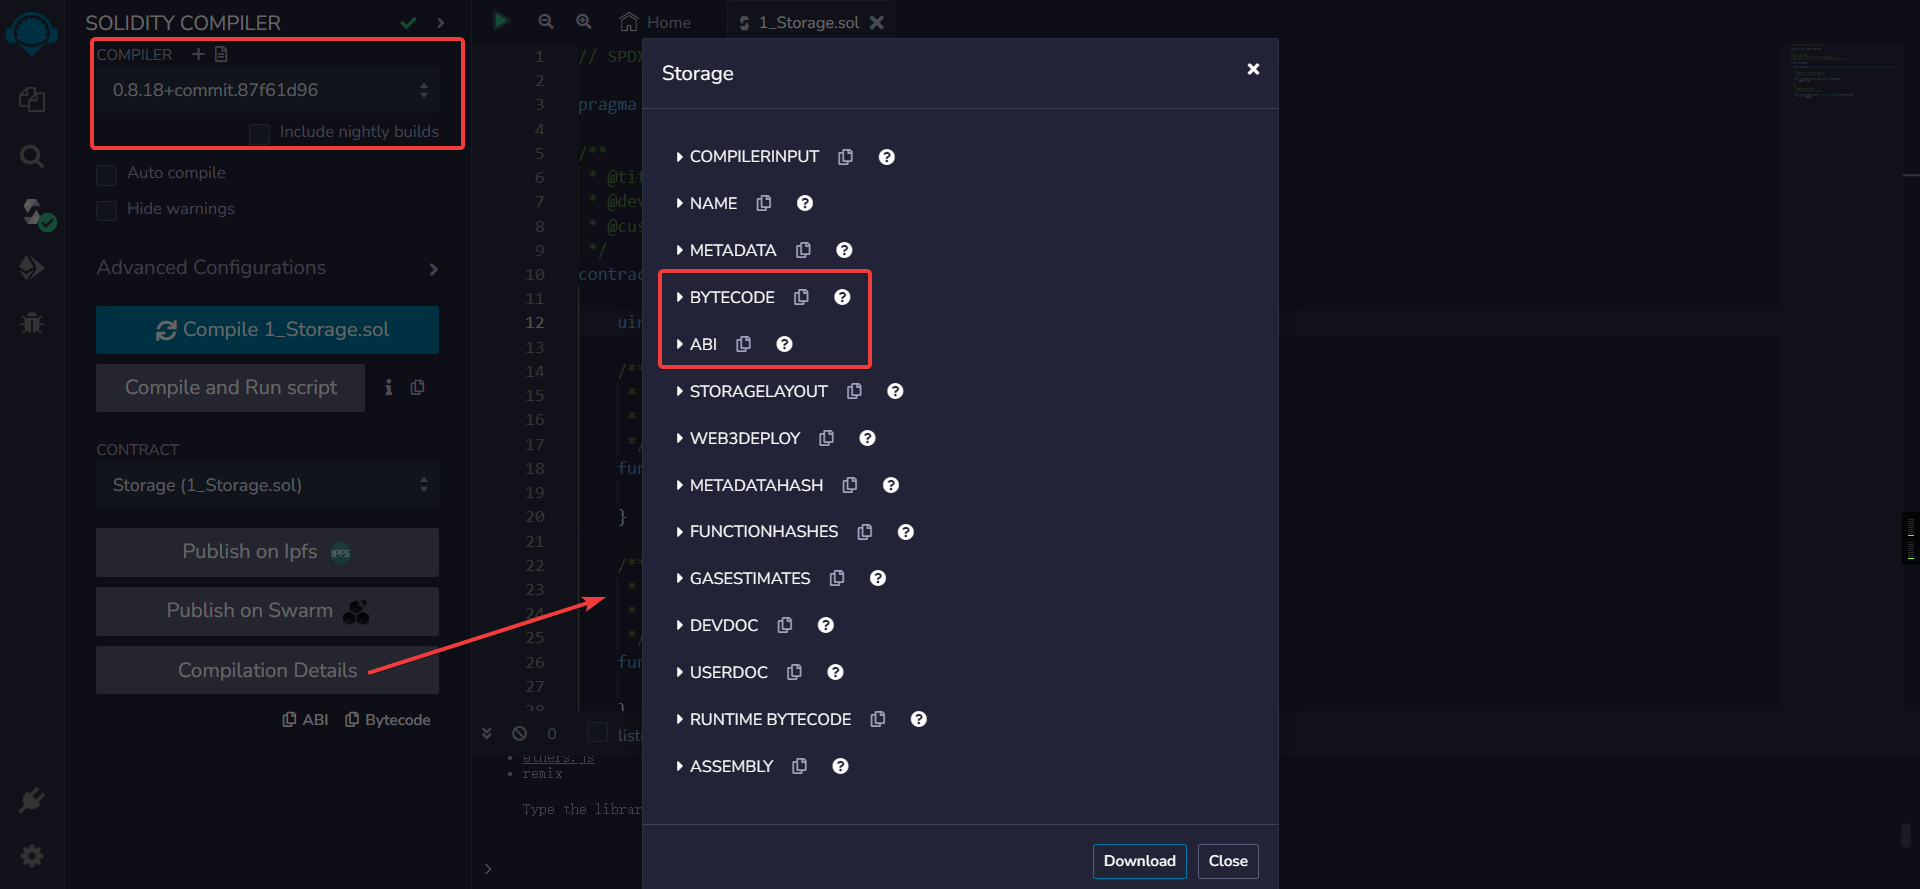
\includegraphics[width=0.8\textwidth]{images/remix.png}
    \caption{Remix IDE编译选项界面}\label{Remix IDE编译选项界面} % label 用来在文中索引
\end{figure}

图中,更靠近中央部分的红框即为部署合约时需要使用的应用程序二进制接口(ABI)和以太坊虚拟机字节码(bytecode)信息,需要妥善记录保存。另外,在合约源代码所在的目录下的artifacts目录中,有一份与合约同名的json文件,该文件亦需要妥善保存备用。

\subsubsection{部署合约}

本文使用附录B中的合约部署模板进行合约部署工作,具体步骤如下:

\begin{enumerate}
    \item 将代码模板中的“经过压缩转义后的ABI”替换为经过压缩转义处理(即:去除多余空格,且为双引号等特殊字符进行转义处理)的上一步骤中获得之应用程序二进制接口
    \item 将“获得的字节码字符串”替换为上一步骤中获得之以太坊虚拟机字节码
    \item 修改变量名Contract、contractInstance为合适的名字,避免多份合约重名
    \item 将经过以上修改的模板代码复制到正在运行geth1的控制台中,单击回车提交部署请求
    \item 使用\verb|miner.start()|开始挖矿,合约地址将随后在终端中显示
\end{enumerate}

需要注意的是,在模板中,可见一名为position的字段。若该字段指代的Geohash在区块链的管辖范围之外(即:区块链管辖的Geohash并非position字段的前缀),将获得out of the blockchain错误,无法继续部署。因此,每次部署前,均需检查position字段指示的范围是否在区块链管辖范围以内。

\subsubsection{合约交互}

部署完成后的合约可以使用合约地址与其建立交互渠道,并调用合约内定义的方法。在web3.js库的辅助下,与合约进行交互仅需短短数行代码。最小示例如下:

\begin{lstlisting}[caption={合约交互}, label={lst:合约交互}]
// 使用web3.js库
const Web3 = require('web3');
// 使用WebSocket协议连接到区块链,本例中端口号为8546
let web3 = new Web3(new Web3.providers.WebsocketProvider("ws://127.0.0.1:8546"));
// 部署合约时获得的合约地址
let contractAddress = '0x23b98f92ceac005e570b6768da377b3abd11012e';
// 编译合约时保存的应用程序二进制接口信息
let contractAbi = JSON.parse(fs.readFileSync('./contractAbi.json', 'utf-8'));
// 合约实例
let contractInstance = new web3.eth.Contract(mapContractAbi, mapContractAddress);
// 调用合约中定义的example方法
contractInstance.methods.example().then((res) => {/* 处理返回值res */});
\end{lstlisting}

在进行实验时,若出现难以排查的错误,应首先考虑合约相关错误。综合上述部署步骤,合约相关错误可以从以下几点进行排查:

\begin{itemize}
    \item 从编译详情处获得的各项数据是否正确?例如,以太坊虚拟机字节码是否与应用程序二进制接口出自同一次编译过程?
    \item 部署合约时,是否正确配置各选项,例如position字段?
    \item 部署完成之后,是否正确记录合约地址?
    \item 进行合约交互前,是否确认区块链允许WebSocket协议连接?部分功能,例如订阅事件,仅能在WebSocket连接下进行。若无,则这些功能可能失效,与合约的交互可能失败。
\end{itemize}

\section{本章小结}

本章介绍了使用区域索引区块链进行基于区块链的出租车调度系统的复现实验之相关工作。首先,简要介绍该调度系统的功能及其组成部分;其次,介绍实验进行的环境配置和包括建立区块链、部署合约、上传地图、前端调试和使用等复现步骤,并展示了复现工作的运行结果,证明了复现工作的正确性;最后,介绍了在进行复现实验时遇到的典型疑难问题,对这些问题进行了产生原因的剖析,给出了解决方法和排查思路。

%%
% The BIThesis Template for Bachelor Graduation Thesis
%
% 北京理工大学毕业设计(论文)第二章节 —— 使用 XeLaTeX 编译
%
% Copyright 2020-2023 BITNP
%
% This work may be distributed and/or modified under the
% conditions of the LaTeX Project Public License, either version 1.3
% of this license or (at your option) any later version.
% The latest version of this license is in
%   http://www.latex-project.org/lppl.txt
% and version 1.3 or later is part of all distributions of LaTeX
% version 2005/12/01 or later.
%
% This work has the LPPL maintenance status `maintained'.
%
% The Current Maintainer of this work is Feng Kaiyu.
%%

\chapter{基于树状区块链的跨链转账测试}

\section{树状区块链的跨链转账}

树状区块链,乃是以区域索引区块链为基础,旨在解决传统区块链单链结构面对大量区块时产生高昂性能代价的痛点。其借助Geohash技术,编码地理位置,并借此对区块链进行划分,形成类似于字典树的树状结构。

然而,这样的结构带来了一个问题:若某个账户的位置发生了较大改变,以至于它离开了目前所在的子链的管辖范围(即账户所在子链表示的Geohash范围不再是账户实际位置的Geohash编码表示的前缀),那么账户在新地理位置上发送的所有交易将失败,因为在逻辑上账户并不由管辖新地理位置所在片区的区块链直接管辖,后者可能根本没有关于该账号的任何记录,或者其上与该账户关联的信息并非切实。

对此,树状区块链的解决方案是:账户需要向一个特殊的管理账号发送一种特殊的交易,该交易及其携带的信息足以令管理账号从账户原先所在的区块链中,将账户的各项信息转移到新区块链上。此后,该账户可以认为由新区块链接手管辖,可以正常进行诸如发送交易等的区块链交互操作。由于上述转账过程与同一区块链内两不同账户间的转账不同,乃是横跨两个区块链的、同一账户之间的转账,故称该特殊转账过程为“跨链转账”。

显然,在尝试解决单链结构的效率问题的同时,树状区块链引入了跨链转账所需的额外时间开销。跨链转账操作的效率,将对用户的使用体验有较大的影响。因此,本章将围绕跨链转账这一主题进行探究。首先,设计并进行数组跨链转账测试实验;其中,以较小规模的10账号跨链转账实验测试跨链转账的正确性;验证正确性后,再开展更大规模的跨链转账测试,检验跨链转账操作在不同压力情况下的运行效率波动;最后,给出一个简单的数学模型,探究树状区块链跨链转账代价与其链上数据查询复杂度降低带来的性能优势基本持平时的临界条件,进而给出适用树状区块链代替传统单链结构区块链的应用场景建议。

\section{设计测试}

跨链转账测试实验将在如图3-1所示的区块链网络中进行。

\begin{figure}[htbp]
    \centering
    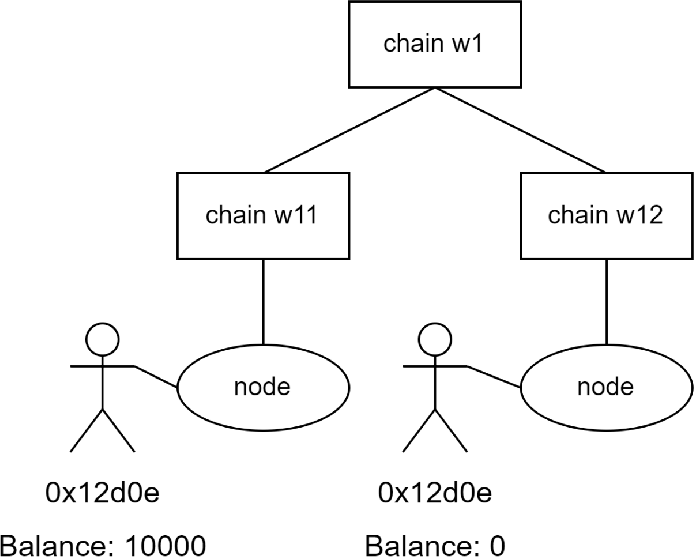
\includegraphics[width=0.8\textwidth]{images/2leaf-structure.png}
    \caption{2leaf结构}\label{2leaf结构} % label 用来在文中索引
\end{figure}

该区块链网络共由三个链组成,分别以链w1,链w11和链w12指代。链w1为树状区块链中的分支区块链,其管辖的地理位置范围为Geohash编码为w1的所有区域;由链w1负责串联的子链w11、子链w12均为叶子区块链,分别管辖Geohash编码前缀为w11、w12的所有区域,其下分别运行有一个节点,可以同传统区块链节点一样进行挖矿、交易等操作。初始时,两子链中存在相同的数个账号,但w11中的账号均有$5 \times 10^{40}$单位的余额,w12中的账号的余额均为0,模拟账号进行了大范围物理位置变动后。管辖权仍未移交给管辖新地点的子链的情况。跨链转账开始后,待所有链w11中的账号同时发起转账申请后,树状区块链将开始串行地遍历所有子链w11中的账号,并将它们在链w11的余额全部转移至链w12的对应账号之下。待转账完成之后,检查链w12中各账户的余额,即可证明跨链转账的功能正确性。

在此过程中,监控程序将记录所有账号发起转账申请的时间戳、以及转账完成时的时间戳。通过分析以上数据,即能得到每个账号从串行处理开始至转账完成所花费的总时间,进而在初始待转账账号数量不同时,得出树状区块链在不同工况下的跨链转账效率。

本测试将从10个账号的小规模跨链转账测试开始,测试在小压力工况下跨链转账功能是否运转正常;在此基础上,继续开展20账号,40账号,80账号,120账号,160账号及200账号跨链转账实验,探究面对不同压力工况时树状区块链的性能表现变化。

\section{环境配置}

跨链转账测试的测试环境如下:

\begin{table}[htbp]
    \linespread{1.5}
    \zihao{5}
    \centering
    \caption{跨链转账测试环境}\label{跨链转账测试环境}
    \begin{tabular}{*{5}{>{\centering\arraybackslash}p{6cm}}} \toprule
        中央处理器 & Intel Core i5-12500H      \\
        图形处理器 & Intel Iris Xe 80EU        \\
        内存    & 24GB                      \\
        操作系统  & Ubuntu 22.04.2 LTS        \\
        虚拟机   & VMWare Workstation Pro 17 \\
        \bottomrule
    \end{tabular}
\end{table}

另外,还需安装\verb|make|程序包,并下载树状区块链的源代码\footnote{https://github.com/xyongcn/BlockChain2017/tree/master/src/go-ethereum1.9.12-modify/go-ethereum}。

\section{测试步骤}

\subsection{编译并配置树状区块链}

下载源代码后,在源代码目录启动终端,输入\verb|make geth|,等待编译完成,即能在\verb|build/bin|目录中发现geth二进制可执行文件。将其重命名为geth-tree,并复制到\verb|/usr/local/bin|目录中。

\subsection{进行测试}

代码仓库\footnote{https://gitee.com/endericedragon/transfer-2leaf}给出了构建图3-1所示的区块链网络的数据文件和脚本,并附有一份实验手册。本节将简要介绍测试步骤。

\begin{enumerate}
    \item 确认w1、w11和w12的数据目录中不存在\verb|gethdata/geth|子目录。若存在,则需要将其删除;
    \item 在代码仓库根目录中启动终端,运行\verb|sh w1_init.sh|指令,启动分支区块链w1,并留意形如\verb|INFO [04-10|20:36:48.833] Started P2P networking self="enode://......"|的输出,记录该双引号包裹的字符串;
    \item 在链w11和链w12的预加载脚本中,替换\verb|admin.addPeer()|方法的参数为上一步中记录的字符串
    \item 另启动两个终端,分别执行启动链w11和链w12的脚本,若观察到形如\begin{verbatim}
INFO [04-10|20:54:02.335] Block synchronisation started
---k:aaaaaaaaaaaaw1,v.RegionId:w1,v.Number:1---
---parent.Number:0, branchb.RegionId:w1,ptd:131072---
!!commitBranchBlock[aaaaaaaaaaaaw1][1]--[td:262144]success!!
    \end{verbatim}
          字样,即为子区块链和父区块链同步成功,可以进行下一步骤的实验;
    \item 另启动一个终端,运行\verb|branchnode-remastered.js|脚本。该脚本将监视父区块链w1的日志内容,并根据之运行相应代码,完成转账等操作;
    \item 在链w11和链w12中启动挖矿后,启动一个终端,执行\verb|node transfer_test_step1.js|指令。该指令将从链w11的矿工账号,分别为链上的其他账号转账10000单位的资产作为初始资金,在接下来的步骤中,这些资产将被转移到链w12中的同名账号上;
    \item 确认初始资金全部到位后,执行\verb|node transfer_test_step2.js|,终端中将出现与挖矿提示\verb|line:--handler-TX_request--|不同的输出,等待,直至终端仅输出挖矿提示;
    \item 执行\verb|node query_transfer_time_w11_w12.js|,脚本将访问链w11和链w12上的所有区块,统计其中包含的交易及其详细信息,生成测试结果报告。
\end{enumerate}

\section{测试结果分析}

使用\verb|eth.getBalance(accountAddress)|函数,可以在Geth的JavaScript控制台中年轻松地查看给定账号的余额,进而检查转账是否成功。本章所有测试均已确认在跨链转账结束后,原链w11中各账户的余额均为0,而链w12中的对应账户余额为10000单位,从而证明了跨链转账功能的正确性。

由于测试设计为将账户余额从链w11转账到链w12中,故在生成的测试报告中,仅需关注\verb|tx_request_w12.txt|和\verb|tx_result_w11.txt|文件即可。前者记录了发起转账申请的时间戳,由于所有账号乃是同时发起转账申请,故所有条目的时间戳均相同;后者记录了各账户在链w12真正收到资产的时间戳。根据后者(即\verb|tx_result_w11.txt|文件),可以轻松重建树状区块链串行处理所有账户的顺序,以及处理各个账户分别花费的时间。

\subsection{小规模跨链转账实验结果分析}

本文以10账号参与的跨链转账测试结果作为小规模跨链转账测试的测试结果。根据测试报告内容,所有10个账号均在时间戳1683465655发起转账申请,但在链w12上收到资产的时间戳不同,数据如下:

\begin{table}[htbp]
    \linespread{1.5}
    \zihao{5}
    \centering
    \caption{10账号测试结果}\label{10账号测试结果}
    \begin{tabular}{*{5}{>{\centering\arraybackslash}p{6cm}}} \toprule
        账号公钥地址                                     & 收到资产的时间戳   \\\hline
        0x4461e120a1bcbdc9e08730f59c7e169bac5de38f & 1683465667 \\
        0x59cadf05182c56784b60960159c0fb4d16860d10 & 1683465680 \\
        0x8ed2d00a4ee496e51fab00ddc7561f85186e2a9c & 1683465688 \\
        0x95fcbbba05858b53b829361a052450179d7a62ca & 1683465694 \\
        0xcada164cb319316a133741dbaa1b40fcc8caec52 & 1683465703 \\
        0x1daf02e444bec7fc7fdbbac7704c57d001b19648 & 1683465711 \\
        0x023bc9309e89678b5de3ea084a5a91cc0679dd39 & 1683465720 \\
        0x4d326e5422c48ca1db8695bb59c9a58005a3fb44 & 1683465724 \\
        0x12d0e4381ef94a70a49252e35b9a65fadd3872b9 & 1683465735 \\
        0x0b424be2eb61a4fa045161198754613a93845857 & 1683465743 \\
        0xf41384cb20cd007daea6b0d7eefa3942ac44a3d1 & 1683465750 \\
        \bottomrule
    \end{tabular}
\end{table}

结合发起转账请求之时间戳,可以使用形如附录C的Python代码计算得到树状区块链为每个账户办理转账所花费的时间并可视化,如图3-2所示:

\begin{figure}[htbp]
    \centering
    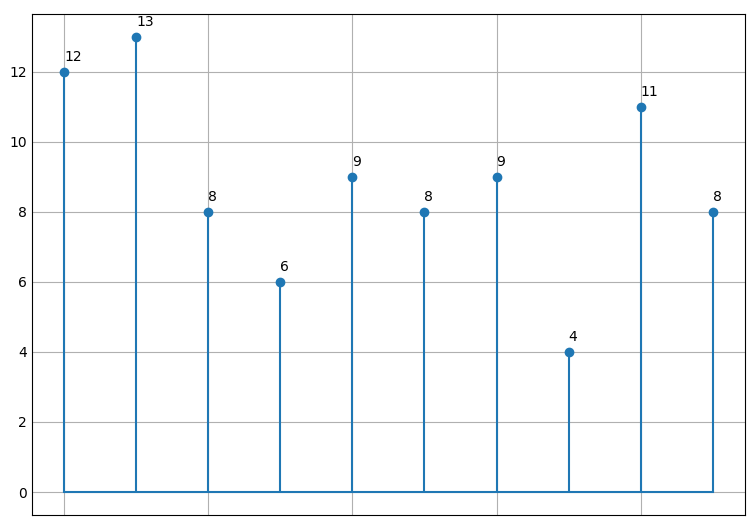
\includegraphics[width=0.8\textwidth]{images/10accounts.png}
    \caption{10账号跨链转账测试的可视化}\label{10账号跨链转账测试的可视化} % label 用来在文中索引
\end{figure}

根据图3-2计算,得到如下测试数据:

\begin{table}[htbp]
    \linespread{1.5}
    \zihao{5}
    \centering
    \caption{10账号测试数据}\label{10账号测试数据}
    \begin{tabular}{*{5}{>{\centering\arraybackslash}p{6cm}}} \toprule
        总耗时(秒)          & 95     \\
        最快转账处理速度(秒)     & 4      \\
        最慢转账处理速度(秒)     & 13     \\
        平均转账处理速度(秒)     & 8.8000 \\
        转账处理速度方差(秒$^2$) & 6.5600 \\
        \bottomrule
    \end{tabular}
\end{table}

观察图3-2不难发现,虽然10个账号的转账申请确实是同时发起的,但由于以太坊仅能串行处理的特性,导致从第一份转账请求发起,到最后一次转账交易完成并写入区块为止的总耗时较为夸张。同时,参与测试的10个账号之转账处理时间方差较大,最快转账处理速度较最慢处理速度的差距足有7秒。

\subsection{大规模跨链转账实验结果分析}

随着请求转账的账号数量增加,其转账处理效率是否会随之变化?本文继续以类似的方法,开展了20账号、40账号、80账号、120账号、160账号、200账号的跨链转账测试。由于篇幅限制,本节将不展示可视化图示,仅展示经过计算得出的统计数据。

\begin{table}[htbp]
    \linespread{1.5}
    \zihao{5}
    \centering
    \caption{测试数据汇总}\label{测试数据汇总}
    \begin{tabular}{r|c|c|c|c|c|c} \toprule
                        & 20账号   & 40账号    & 80账号    & 120账号  & 160账号   & 200账号   \\\hline
        总耗时(秒)          & 163    & 319     & 654     & 978    & 1363    & 1621    \\
        最快转账处理速度(秒)     & 4      & 2       & 1       & 2      & 1       & 1       \\
        最慢转账处理速度(秒)     & 16     & 17      & 21      & 17     & 27      & 21      \\
        平均转账处理速度(秒)     & 9.0556 & 8.6216  & 8.9589  & 8.5789 & 11.2645 & 8.7622  \\
        转账处理速度方差(秒$^2$) & 8.0525 & 11.0460 & 19.0805 & 8.3666 & 25.9446 & 12.8407 \\
        \bottomrule
    \end{tabular}
\end{table}

观察表3-4的数据,可以提出以下猜想:
\begin{itemize}
    \item 转账过程耗时和参与转账的账号存在线性关系;
    \item 虽然转账处理速度方差较大,但平均处理速度较为稳定,大约在8.5秒到11.3秒之间。
\end{itemize}

其中,第二个猜想可以从表3-4中较直观地得到,故本文将重点讨论第一个猜想的验证。

\subsubsection{验证转账耗时和账号数量的线性关系}

本文使用最小二乘法进行线性拟合计算。记账号数量为$x$,假设$time_\theta(x)$为$x$个账号跨链转账需要花费的时间,那么后者可以写作:

$$
    time_\theta(x) =
    \begin{bmatrix}
        1 & x \\
    \end{bmatrix}
    \cdot
    \begin{bmatrix}
        \theta_0 \\
        \theta_1
    \end{bmatrix}
$$

根据最小二乘法:

$$
    \vec{\theta} = (\vec{X}^T \vec{X})^{-1}\vec{X}^T \cdot \vec{Y}
$$

其中,$\vec{X}$,$\vec{Y}$是分别为样本的输入向量和输出向量。根据以上算法,可得本例中的各个向量为:

$$
    \vec{X} = \begin{bmatrix}
        1 & 20 \\ 1 & 40 \\ 1 & 80 \\ 1 & 120 \\ 1 & 160 \\ 1 & 200
    \end{bmatrix} \\
    \vec{Y} = \begin{bmatrix}
        163 \\ 319 \\ 654 \\ 978 \\ 1363 \\ 1621
    \end{bmatrix}
$$

带入最小二乘法公式进行计算,可得:

$$
    \theta = \begin{bmatrix}
        -4.68767123 \\
        8.26794521
    \end{bmatrix} \\
$$
$$
    R^2 = 1 - \frac{\sum_i (y_i - \overline{y})^2}{\sum_i (y_i - times_{theta}(x_i))^2} = 0.9982362552443657
$$

其中,$x_i$,$y_i$代表$\vec{Y}$的各个水平分量,$\overline{y}$代表$\vec{Y}$的算术平均值。

拟合度$R^2$非常接近1,这正证明了自变量——账号数量$x$和因变量——跨链转账耗时$time_theta$确实可以在统计学上认为存在线性关系$time_{\theta}(x) = -4.68767123 + 8.26794521 \cdot x$,进而验证了以太坊顺序串行处理收到的所有交易的特点。

\section{基于测试结果进行数学建模}

传统区块链单链结构的查询效率低,但胜在无需额外操作维护正确的账户状态;而树状结构的查询效率高,但引入了跨链转账的额外开销。根据使用场景的不同,用户需要在上述两种区块链实现中恰当进行选择,方能在特定的应用场合获得更好的使用体验。本节将基于已收集的测试数据,建立简单的数学模型,探讨在不同场景下使用树状区块链和传统区块链的理论性能差异,为用户在两种区块链实现之间的选择提供建议。

\subsection{静态查询复杂度分析}

静态查询复杂度分析,约束所有账号的地理位置不发生变化,因此不会考虑跨链查询的情况。本小节将基于以上约束,讨论单链结构区块链和树状区块链查询信息的复杂度情况。

在单链结构区块链下,所有链上信息均存储在同一条链中。若进行一次查询,最坏情况下需要遍历整条链才能获得结果。记总区块数为$n$,则该过程的平均时间复杂度为$O(n)$。

在树状区块链下,情况较为复杂,为简单起见,本节讨论一条父链,$x$条子链组成的双层树状区块链,并假设所有区块均匀地分布在子链中。仍记总区块数为$n$,那么每条子链中包含$\frac{n}{x}$个区块。此时若进行一次查询,最坏情况下仅需遍历一条子链即可,平均时间复杂度为$O(\frac{n}{x})$。

注意到当分母$x$越大,查询的时间复杂度越低。这是因为,在区块均匀分布的前提下,数状结构的深度随分支的增加而减少。结合树状区块链分支的实际意义,可以得到以下结论:

\begin{itemize}
    \item 当链上交易发生的地理位置跨度较大,且在各地理位置范围分布较均匀时,适合使用树状区块链而非单链结构区块链;
    \item 当链上交易发生的地理位置非常集中时,树状区块链的表现和单链结构区块链接近,故无需使用树状区块链。
\end{itemize}

\subsection{动态查询复杂度分析}

动态查询复杂度分析,假设节点在树状区块链的各子链间周期性移动,从而将跨链这一开销纳入考量。本小节中,将针对节点中的一个账号进行分析。该账号行为描述如下:处于某一条子链中时,进行数笔交易,这些交易分别记录在不同的区块中。随后,账号立即转移前往下一个子链,此时若进行查询操作,必须先进行跨链转账,将该账户之余额转移到新子链上,然后再进行查询。

在单链结构区块链下,情况与静态查询情况类似,进行一次查询,最坏情况下仅需遍历一条子链即可,平均时间复杂度为$O(n)$。

在树状区块链下,情况更为复杂。记$lcm(c, q)$为账号跨链的间隔之间产生的区块数量$q$和查询间隔之间产生的区块数$c$的最小公倍数,那么在产生$lcm(c, q)$个区块的过程中,将发生$\frac{lcm(c, q)}{c}$次查询,且账号将进行$\frac{lcm(c, q)}{q}$次跨链移动。那么$\frac{lcm(c, q)}{c}$次查询的总时间复杂度为$O(q \times \frac{lcm(c, q)}{c}) + \frac{lcm(c, q)}{q} \times T_{cross}$,其中$T_{cross}$为单个账户跨链转账的时间开销。那么,平均到每一次查询的时间开销即为$(O(q \times \frac{lcm(c, q)}{c}) + \frac{lcm(c, q)}{q} \times T_{cross}) \times \frac{c}{lcm(c, q)} = O(q) + \frac{c}{q} \times T_{cross}$。

令$lcm(c, q) = n$,比较两区块链实现在生成相同区块数量下的复杂度表现,列不等式:

$$
    O(lcm(c, q)) \geq O(q) + \frac{c}{q} \times T_{cross}
$$

由于在遍历长为$length$的区块链链条时,可以认为找到目标区块的期望复杂度为$\frac{length}{2}$;同时,经过实测,$T_{cross}$的值可以取表3-4中跨链转账测试的平均处理速度的平均值(经过计算,为大约9.2070秒),故可以改写上述不等式为:

$$
    \frac{lcm(c, q)}{2} \geq \frac{q}{2} + \frac{c}{q} \times 9.2070
$$

当满足上述不等式时,树状区块链才可能提供相较传统区块链更优越的性能。

观察树状区块链的动态查询复杂度表达式可知,当查询非常频繁,即$c$的值变小时,复杂度将相应降低。

注意到,$q$的增大在$O(q)$中,对时间复杂度起到增加作用,却在$\frac{c}{q} \times acc \times T_{cross}$中起到减少时间复杂度的作用。这是因为,增大$q$相当于容许子链拥有更长的长度,节点停留在同一子链中的时间延长,也就相应减少了跨链转账操作的次数。因此,即便是在树状区块链中,用户也需要合理设计子链的管辖范围,将节点跨链的频率控制在合理的区间内。

综上所述,在下列场景中,选择树状区块链将比选择单链结构区块链更优:

\begin{itemize}
    \item 账号的物理位置变化范围不太大;
    \item 数据查询请求量较大。
\end{itemize}

\section{本章小结}

本章介绍了树状区块链为保证子链间数据一致性而生的新概念——跨链转账操作,介绍了该操作引入的额外时间复杂度。随后,设计并进行了一系列测试,按照压力自小到大的顺序逐步验证了跨链转账操作的结果正确性、具体测量了该操作带来的额外时间开销,将其可视化并统计整理,进行统计学分析。在分析时,发现并合理利用一些最优化方法验证了参与转账的账户数量与转账耗时的线性关系,证明跨链转账这一操作为串行处理。最后,分别在静态和动态的场景下建立简单的数学模型,从理论与实际测量数据结合的角度比较了传统单链结构区块链和树状区块链的性能表现,并就在何场景下使用何者给出了一些建议。

%%
% The BIThesis Template for Bachelor Graduation Thesis
%
% 北京理工大学毕业设计(论文)第二章节 —— 使用 XeLaTeX 编译
%
% Copyright 2020-2023 BITNP
%
% This work may be distributed and/or modified under the
% conditions of the LaTeX Project Public License, either version 1.3
% of this license or (at your option) any later version.
% The latest version of this license is in
%   http://www.latex-project.org/lppl.txt
% and version 1.3 or later is part of all distributions of LaTeX
% version 2005/12/01 or later.
%
% This work has the LPPL maintenance status `maintained'.
%
% The Current Maintainer of this work is Feng Kaiyu.
%%

\chapter{以出租车调度系统为背景的树状区块链测试}

\section{树状区块链上的出租车调度系统测试简介}

树状区块链将单链结构转化为树状结构的改进,提升了区块链技术在地理位置有关的应用场景下的理论效率。但实验室尚未对树状区块链在实际应用环境中的表现进行测试。因此,测试树状区块链在实际应用中的真实性能,证明其相较传统单链结构区块链具有可观性能提升的工作迫在眉睫。本章将以实验室已有工作——基于区块链的出租车调度系统为应用背景,以第二章的该系统的复现实验为基础,使用geth1和geth-tree分别构建不同拓扑结构的区块链并于其上运行该调度系统,统计在一定压力负载下司机侧和乘客侧各关键节点的时间戳并将结果可视化,以测试树状区块链在实际应用场景中的性能表现。同时,重构已有脚本的代码,增强其可扩展性和易用性,方面后人进行本测试的复现。

\section{测试设计思路}

本测试分为基于树状区块链geth-tree的测试和基于区域索引区块链geth1的测试两部分,用以对比两种区块链实现在同一套系统下的性能表现差异。

两部分实验中均在真实世界地图中Geohash编码前缀为wx4e的区域下进行。树状区块链部分的实验在该区域下的细分区域wx4en、wx4ep、wx4eq和wx4er区域下进行。每个区域中,均存在16位司机和32位乘客,所有司机的初始位置均相同,所有乘客的出发地点和目的地也相同。以上地点的选点工作基于蒙思洁完成的真实地图信息提取与筛选工作进行,已提前确保选择的路线可以在真实世界地图上导航成功。

本测试使用JavaScript脚本模拟司乘交互行为。司机模拟脚本负责读取司机的公钥地址、初始位置,并将其上传到链上;随后,司机将监听一系列合约中定义的事件,例如乘车请求事件、乘客上车事件和付款事件等,并作出接单、导航、设置车辆状态等响应。乘客模拟脚本负责读取乘客的公钥地址、起始点位置和目的地位置,并将其上传到链上;每隔一段时间(在树状区块链中为3秒,在区域索引区块链中为前者的$\frac14$),将有一名乘客发射乘车请求事件。发射乘车请求事件后乘客将在临近区域周边搜索与自身曼哈顿距离最近的车辆并尝试占有。若车辆已被占用,则等待一段时间(等待时间为冲突次数的一次函数)后再次重复上述步骤,直至车辆分配成功。乘客端、司机端的模拟脚本运行逻辑可分别用图\ref{乘客端模拟脚本运行逻辑}、图\ref{司机端模拟脚本运行逻辑}所示之流程图表示。

\begin{figure}[htbp]
    \centering
    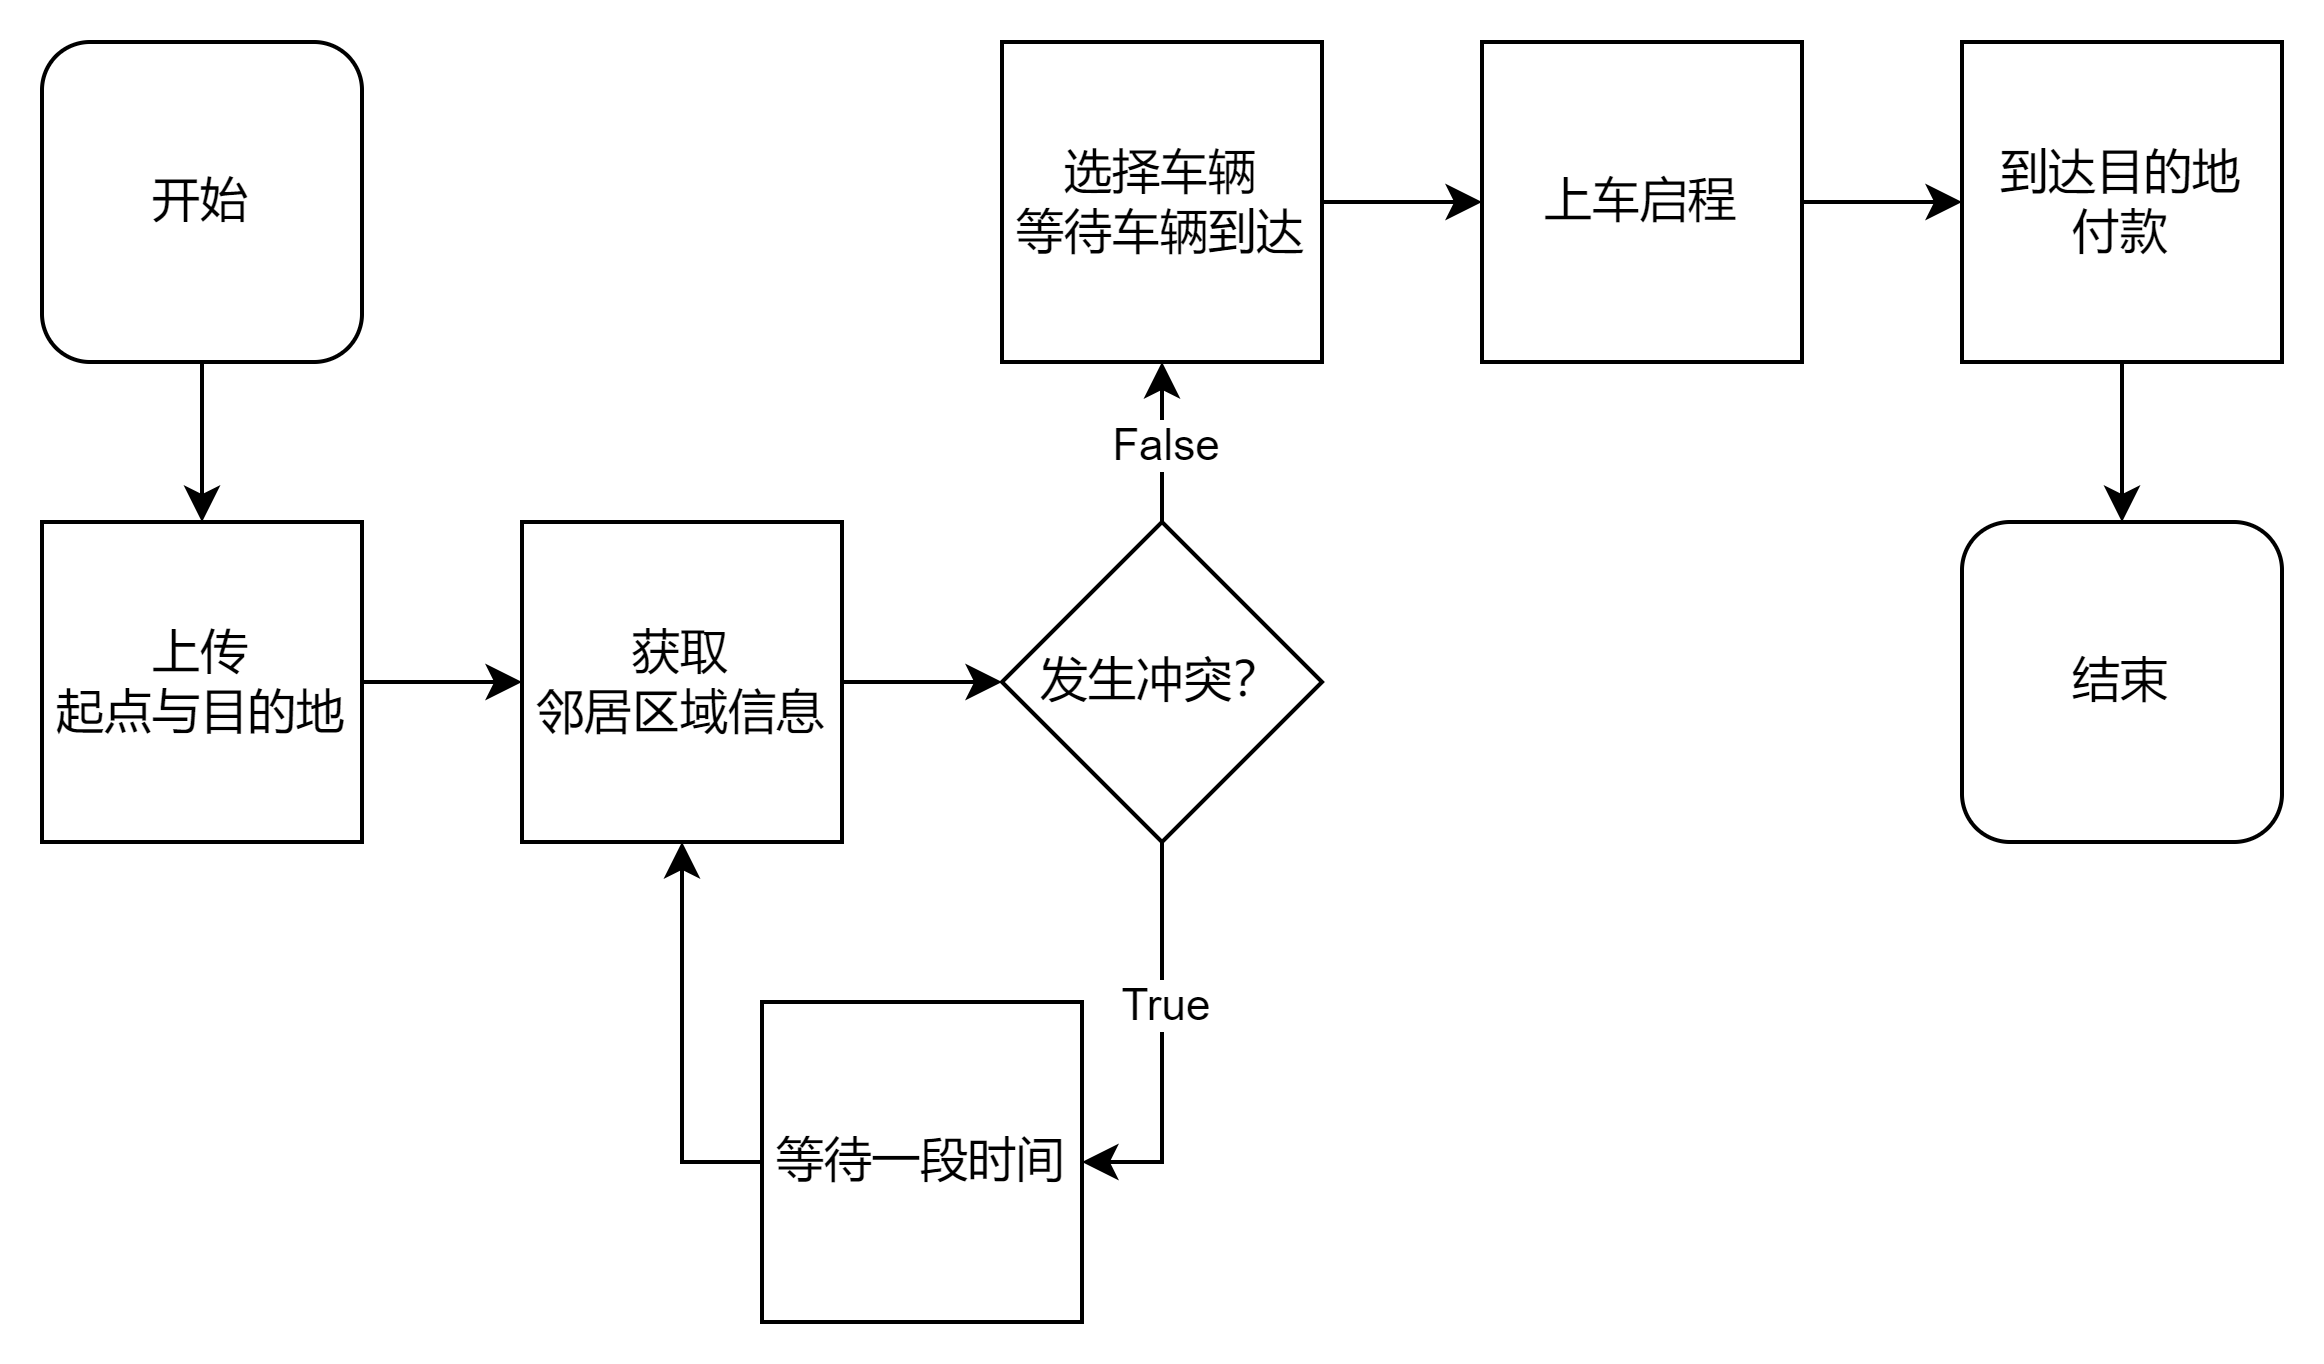
\includegraphics[width=\textwidth]{images/passenger示意图.png}
    \caption{乘客端模拟脚本运行逻辑}\label{乘客端模拟脚本运行逻辑} % label 用来在文中索引
\end{figure}

\begin{figure}[htbp]
    \centering
    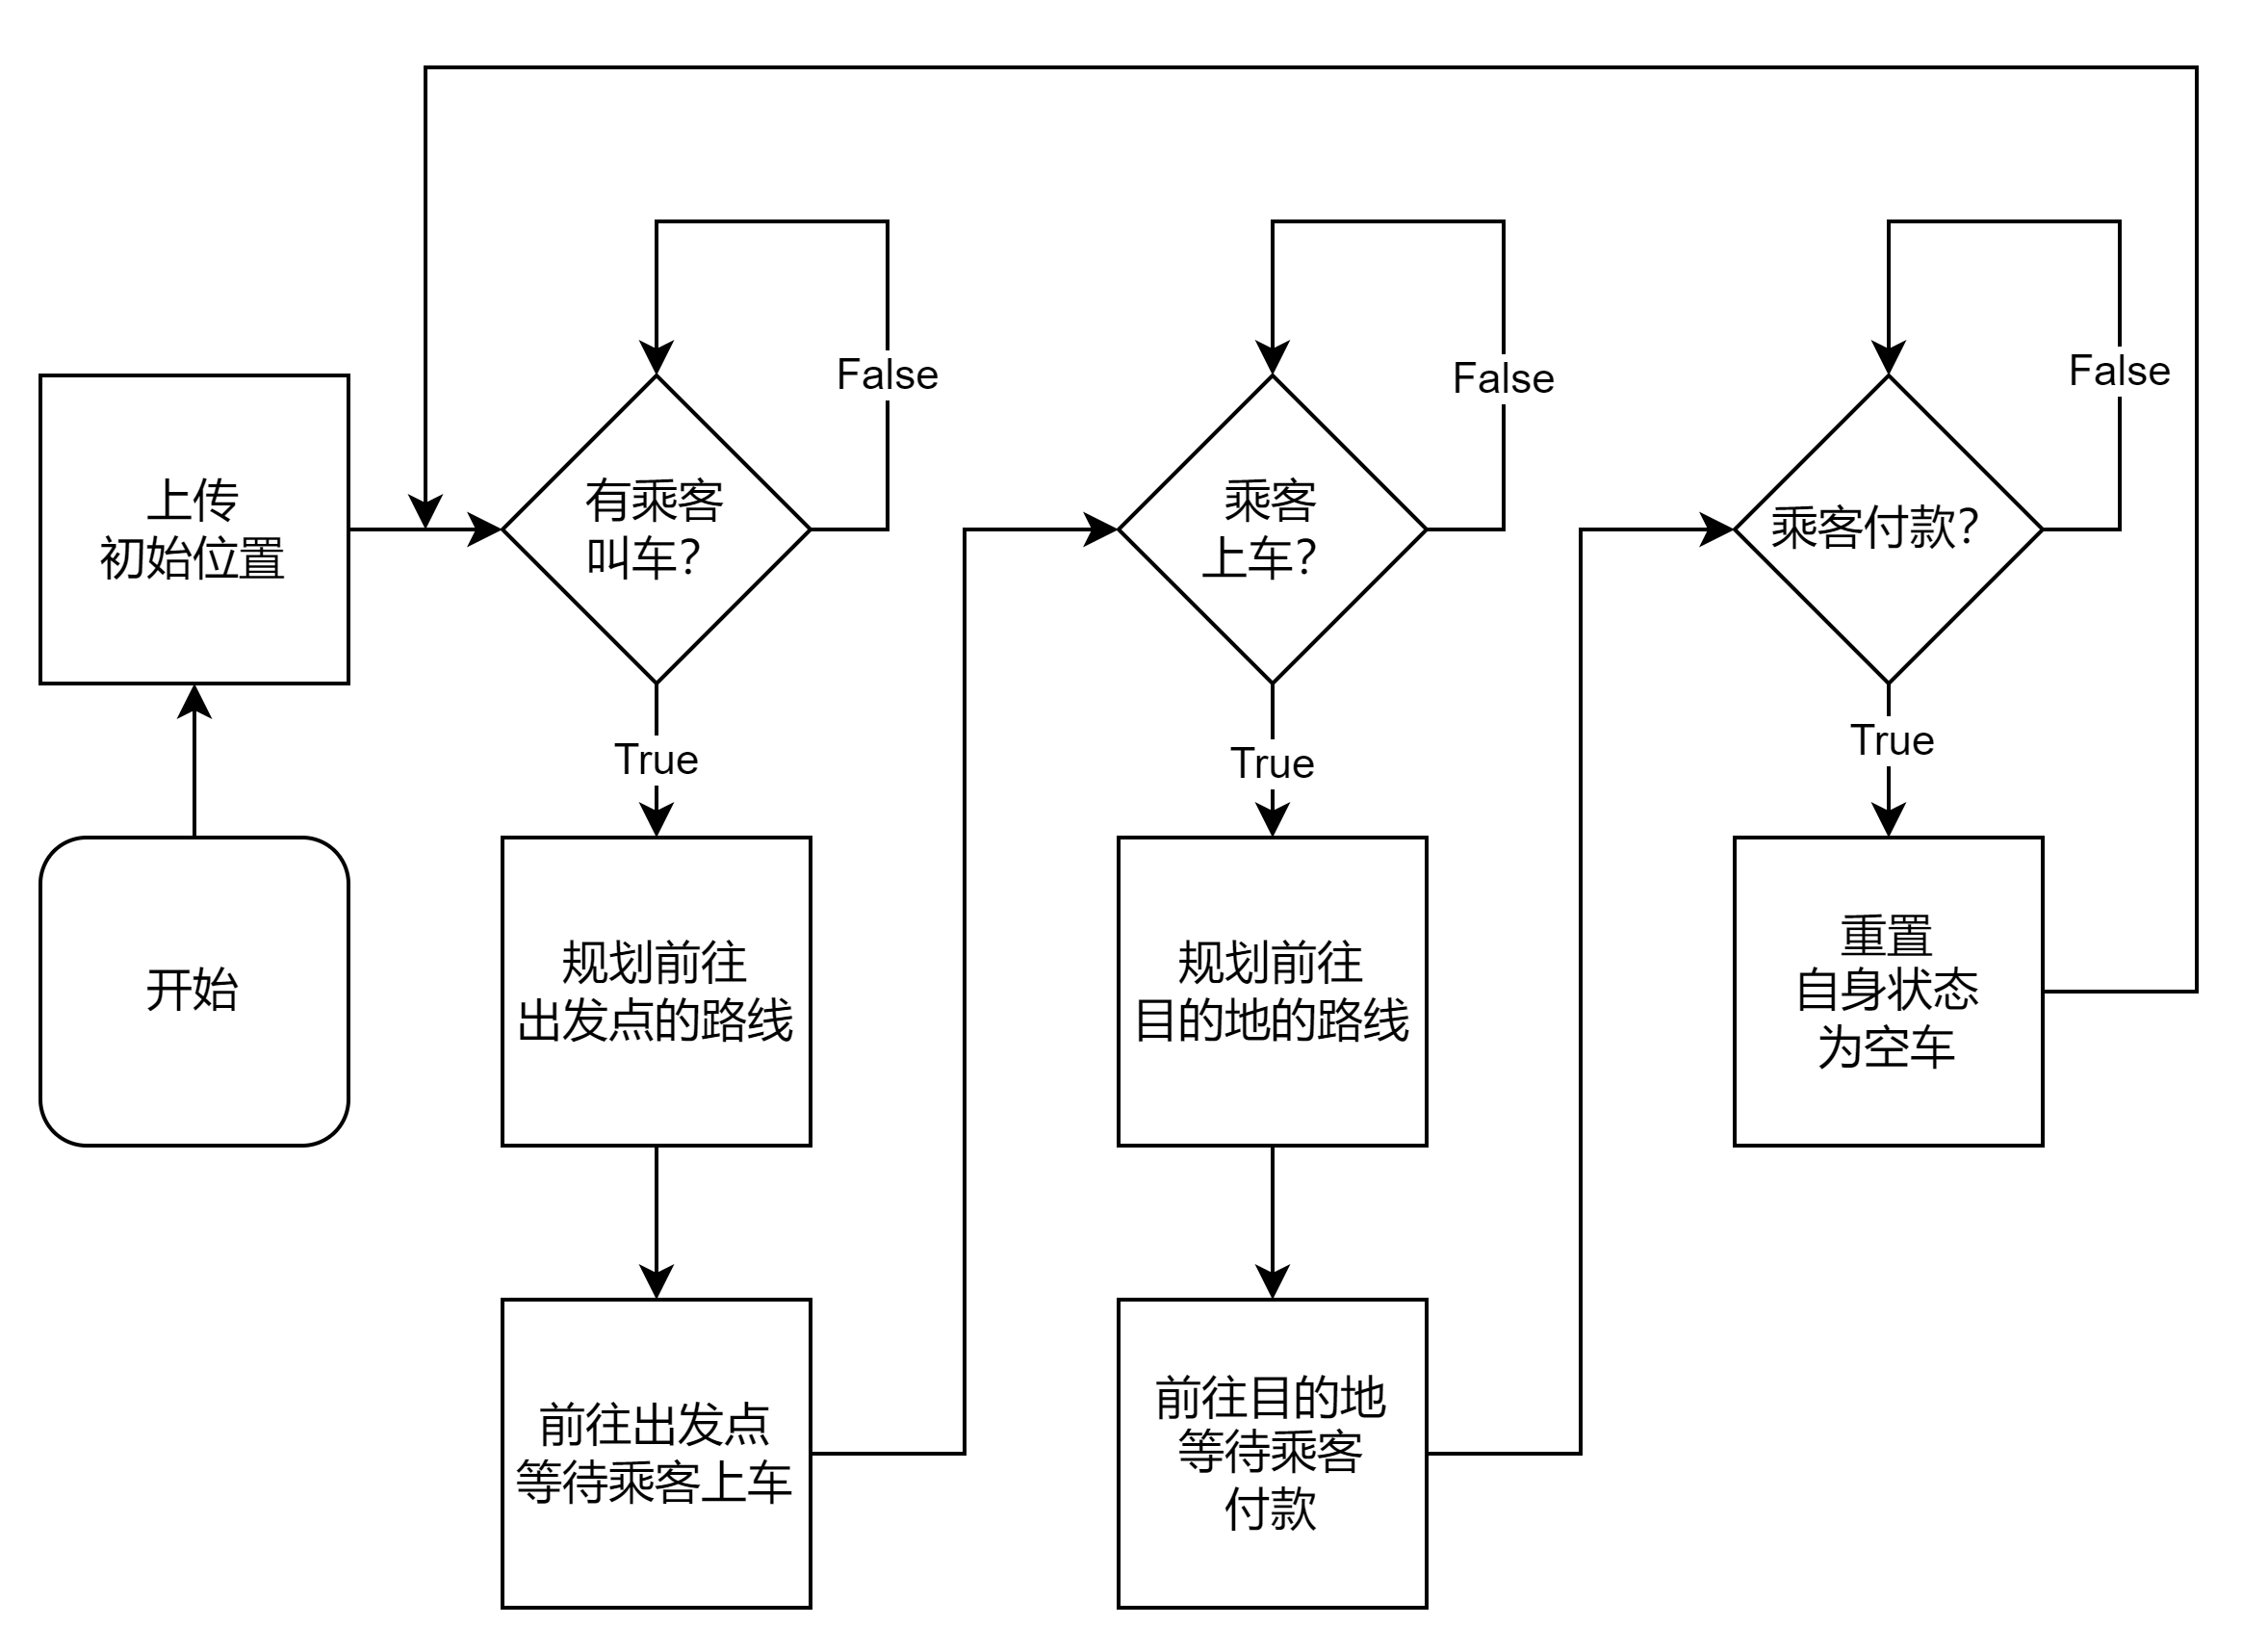
\includegraphics[width=\textwidth]{images/vehicle示意图.png}
    \caption{司机端模拟脚本运行逻辑}\label{司机端模拟脚本运行逻辑} % label 用来在文中索引
\end{figure}

进行树状区块链部分的实验时,首先搭建树状结构,在每个子链上分别部署合约。待合约部署完毕后,所有子链同时挖矿,并同时运行模拟司乘交互行为的JavaScript脚本,该脚本读取对应子链管辖的细分区域内的司乘信息,并记录司乘双方各自在调度过程关键节点的时间戳。

在区域索引区块链测试部分中,测试步骤大致相同,但运行司乘交互模拟脚本时,应令其读取所有四个细分区域内所司乘的信息,模拟不进行区域细分,使用单链结构区块链运行出租车调度系统的应用场景。

\section{测试环境}

基于树状区块链的调度系统测试在表\ref{树状区块链调度系统测试环境}环境中进行。由于运行四子链的性能开销较大,笔者使用Windows下的Linux子系统(WSL 2)代替虚拟机,以提升开发体验。

\begin{table}[htbp]
    \linespread{1.5}
    \zihao{5}
    \centering
    \caption{树状区块链调度系统测试环境}\label{树状区块链调度系统测试环境}
    \begin{tabular}{r|l} \toprule
        中央处理器 & Intel Core i5-12500H      \\
        图形处理器 & Intel Iris Xe 80EU        \\
        内存    & 24GB                      \\
        操作系统  & Ubuntu 22.04.2 LTS        \\
        虚拟机   & Windows Subsystem Linus 2 \\
        \bottomrule
    \end{tabular}
\end{table}

\section{准备数据}

\subsection{确定司乘位置信息}

本节将分别在各树状区块链子链的管辖区域内,为接下来的测试选择一条能够导航成功的路线,其始端和终端分别作为乘客的起点与目的地;司机的初始位置,则设置为乘客的目的地,即导航路线的终端。经过挑选和在调度系统中的验证工作后,笔者最终选择表\ref{测试数据集选点}中所示之点位,作为本章测试的测试数据集。

\begin{table}[htbp]
    \linespread{1.5}
    \zihao{5}
    \centering
    \caption{测试数据集选点}\label{测试数据集选点}
    \begin{tabular}{c|c|c|c} \toprule
        区域Geohash前缀 & 乘客起点        & 乘客终点        & 司机初始位置      \\\hline
        wx4en       & wx4enscgue5 & wx4enrq9mm9 & wx4enrq9mm9 \\
        wx4ep       & wx4epb8scg1 & wx4ep8e5gw0 & wx4ep8e5gw0 \\
        wx4eq       & wx4eq7rgmxk & wx4eqt6u0vu & wx4eqt6u0vu \\
        wx4er       & wx4erd4xkyz & wx4erw9rmze & wx4erw9rmze \\
        \bottomrule
    \end{tabular}
\end{table}

\subsection{划分账号扮演的角色}

基于区块链的出租车调度系统中,账号可以扮演司机或乘客角色。本测试共有192个账号参与其中,且司机角色与乘客角色的数量之比为$1:2$。不仅如此,测试还需保证在四条子链中包含相同数量的司机账号和乘客账号,以维护子链之间的测试公平性。经过计算,本测试将如表\ref{测试账号角色划分}所示,对链上创建的共计192个账号(表中以\verb|eth.accounts|指代)进行划分,该划分方案恰好满足所有子链包含相同数量的乘客账号和司机账号的测试需求。

\begin{table}[htbp]
    \linespread{1.5}
    \zihao{5}
    \centering
    \caption{测试账号角色划分}\label{测试账号角色划分}
    \begin{tabular}{l|l|l} \toprule
        区域Geohash前缀 & 司机账号                                & 乘客账号                                \\\hline
        wx4en       & \verb|eth.accounts.slice(0, 16)|    & \verb|eth.accounts.slice(16, 48)|   \\
        wx4ep       & \verb|eth.accounts.slice(48, 64)|   & \verb|eth.accounts.slice(64, 96)|   \\
        wx4eq       & \verb|eth.accounts.slice(96, 112)|  & \verb|eth.accounts.slice(112, 144)| \\
        wx4er       & \verb|eth.accounts.slice(144, 160)| & \verb|eth.accounts.slice(160, 192)| \\
        \bottomrule
    \end{tabular}
\end{table}

上述划分方案及各账号相关的位置信息将以JSON格式存储到文件,供模拟运行脚本读取之用。

\section{进行模拟运行测试}

本节的详细测试步骤已记录于在线代码仓库\footnote{\url{https://gitcode.net/qq_39710999/taxi-4-leaves}},故本节仅简要介绍大致测试方法。

\begin{enumerate}
    \item 准备司乘数据,使用JSON格式存储每位司乘的信息,并将其均匀分作4份,作为树状区块链子链的测试数据;同时,准备一套存储完整司乘信息的文件,作为区域索引区块链的测试数据;
    \item 建立有四个子链的树状区块链网络,确保四个子链中均拥有相同的192个账号,并已经为它们执行解锁操作;
    \item 在四子链上分别部署合约,并使用得到的合约地址更新各脚本中存储的合约地址,随后上传地图;
    \item 依次启动子链挖矿,注意分配CPU核心数量相同以控制变量,随后选择冲突等待时间和冲突次数的一次函数为$t_{waiting} = 10000 + 4000 \times count$,其中$count$为冲突次数,编辑模拟司机与乘客交互行为的脚本后启动之,等待测试结束;
    \item 模拟脚本运行结束后,将生成测试报告,可对其进行数据处理和可视化;
    \item 建立仅包含一个节点的区域索引区块链网络,于其上进行相似的测试。
\end{enumerate}

\section{乘客端测试数据分析}

本节采用Python 3编程语言的MatPlotLib库作为数据可视化工具,从乘客端方面对收集的测试数据进行分析。

本测试统计三个指标:乘车请求提交耗时、车辆分配耗时和到达并付款耗时。上述三个指标与图4-1中的对应关系如下:

\begin{itemize}
    \item 乘车请求提交耗时:从“开始”开始计时,直至第一次执行“发生冲突?”检查的耗时;
    \item 车辆分配耗时:从第一次执行“发生冲突?”检查开始,直至运行至“选择车辆 等待车辆到达”的耗时;
    \item 到达并付款耗时:从“选择车辆 等待车辆到达”开始计时,直至“结束”的耗时。
\end{itemize}

应用上述指标规则,对乘客端测试数据进行计算和可视化处理,其可视化结果如图\ref{乘客端耗时对比(子链并行运行)}所示所示。

\begin{figure}[htbp]
    \centering
    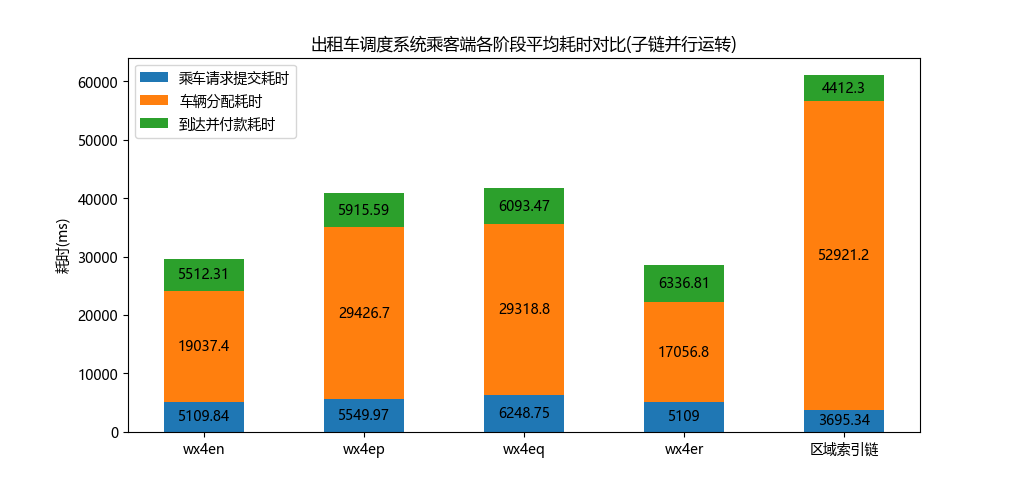
\includegraphics[width=\textwidth]{images/乘客端测试-并行.png}
    \caption{乘客端各阶段平均耗时对比(子链并行运转)}\label{乘客端耗时对比(子链并行运行)} % label 用来在文中索引
\end{figure}

分析图\ref{乘客端耗时对比(子链并行运行)}可知,树状区块链在为乘客分配车辆时,展现出了更为优越的性能。在该阶段中,树状区块链最快用时约17056.8毫秒即完成车辆分配,四子链平均车辆分配时间为23709.9毫秒;相比之下,区域索引区块链共耗时52921.2毫秒完成车辆分配,耗时增长至前者的2.23倍。

进一步分析测试报告发现,区域索引区块链上发生的冲突次数远远大于树状区块链中的各条子链上的冲突次数,是拖慢调度系统在其上运行速度的主要原因。测试报告指出,在区域索引区块链上,一共发生了266次这样的冲突事件;作为对比,冲突事件在wx4en子链、wx4ep子链、wx4eq子链和wx4er子链中的发生次数分别仅有18、31、33、12次,远低于区域索引区块链上的冲突次数。

\subsection{减少无关变量后的补充测试}

注意到,乘客方提交乘车请求、到达目的地并支付路费时,其处理速度相较区域索引区块链并未展现出更高的效率,耗时甚至不降反升。由于测试时四条子链并行运行,且笔者观察到测试时计算机中央处理器负载极高,一度达到满载,故做出如下合理推测:四条子链并行的测试方法极有可能受到测试机器性能上限之影响,从而引入无关变量,令测试数据失真。

为缓解测试机器性能上限对测试结果的影响,笔者补充进行了四次树状区块链实验,每次实验中,仅有一条子链单独运行模拟运行测试,其余三条子链空闲无负载。使用新方法重新测试后,子链的性能表现有了极大的提升,如图\ref{乘客端耗时对比(子链独立运行)}所示。

\begin{figure}[htbp]
    \centering
    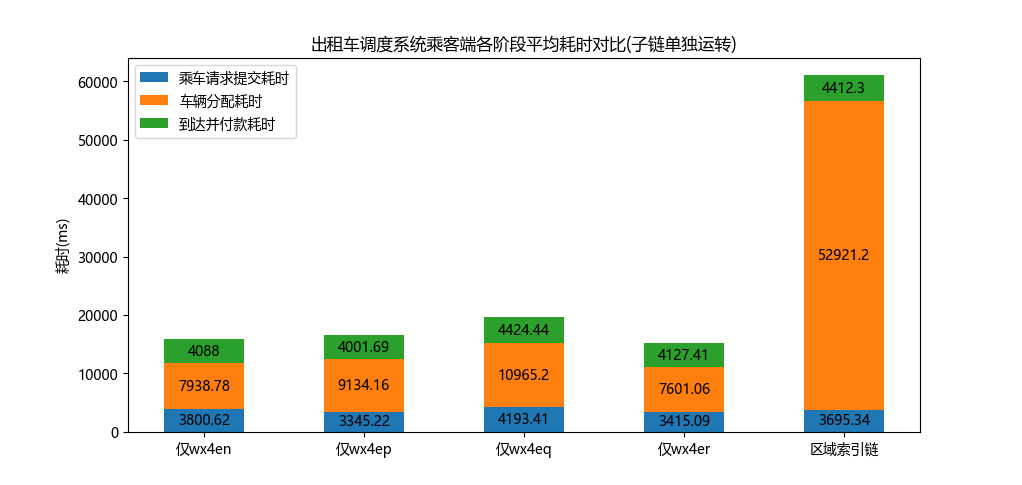
\includegraphics[width=\textwidth]{images/乘客端测试-独立.png}
    \caption{乘客端各阶段平均耗时对比(子链单独运转)}\label{乘客端耗时对比(子链独立运行)} % label 用来在文中索引
\end{figure}

在各个子链独立运行的场景下,测试机器的性能上限带来的影响进一步减弱,此时树状区块链爆发出了远超区域索引区块链的性能表现。在乘车请求提交平均耗时方面,树状区块链与区域索引区块链在该阶段的平均耗时基本一致;在车辆分配耗时方面,四条子链的平均耗时为8909.8毫秒,相较四子链并行运行的工况减少了62.4\%,相比区域索引区块链,其时间开销更是缩短到原来的16.8\%。在到达并付款耗时方面,由于调度系统运行至该阶段时,链上存在的区块数量已较有规模,树状区块链将区块分散至子链以换取更高的处理速度的优势得以提现,此时,四条子链的平均时间消耗为4160.4毫秒,以251.9毫秒的优势领先区域索引区块链。

\section{司机端测试数据分析}

本节使用与上一节相同的工具,对司机端方面进行测试数据分析。

本测试统计三个指标:接单并导航至上车点耗时、导航至目的地耗时和确认乘客下车并付款耗时耗时。上述三个指标与图\ref{乘客端模拟脚本运行逻辑}中的对应关系如下:

\begin{itemize}
    \item 接单并导航至上车点耗时:从“有乘客叫车”检查为真开始,至“前往出发点等待乘客上车”的耗时;
    \item 导航至目的地耗时:从“乘客上车”检查为真开始,至“前往目的地等待乘客付款”的耗时;
    \item 确认乘客下车并付款耗时:从“乘客付款”检查为真开始,至“重置自身状态为空车”为止。
\end{itemize}

应用上述指标规则,对司机端测试数据进行统计和可视化处理。此处沿用了乘客端测试的方法,同时测试了在四条子链并行运转和分别运转的工况下调度系统的运行情况。经过处理和汇总的数据可视化结果如图\ref{司机端平均耗时对比}所示所示。

\begin{figure}[htbp]
    \centering
    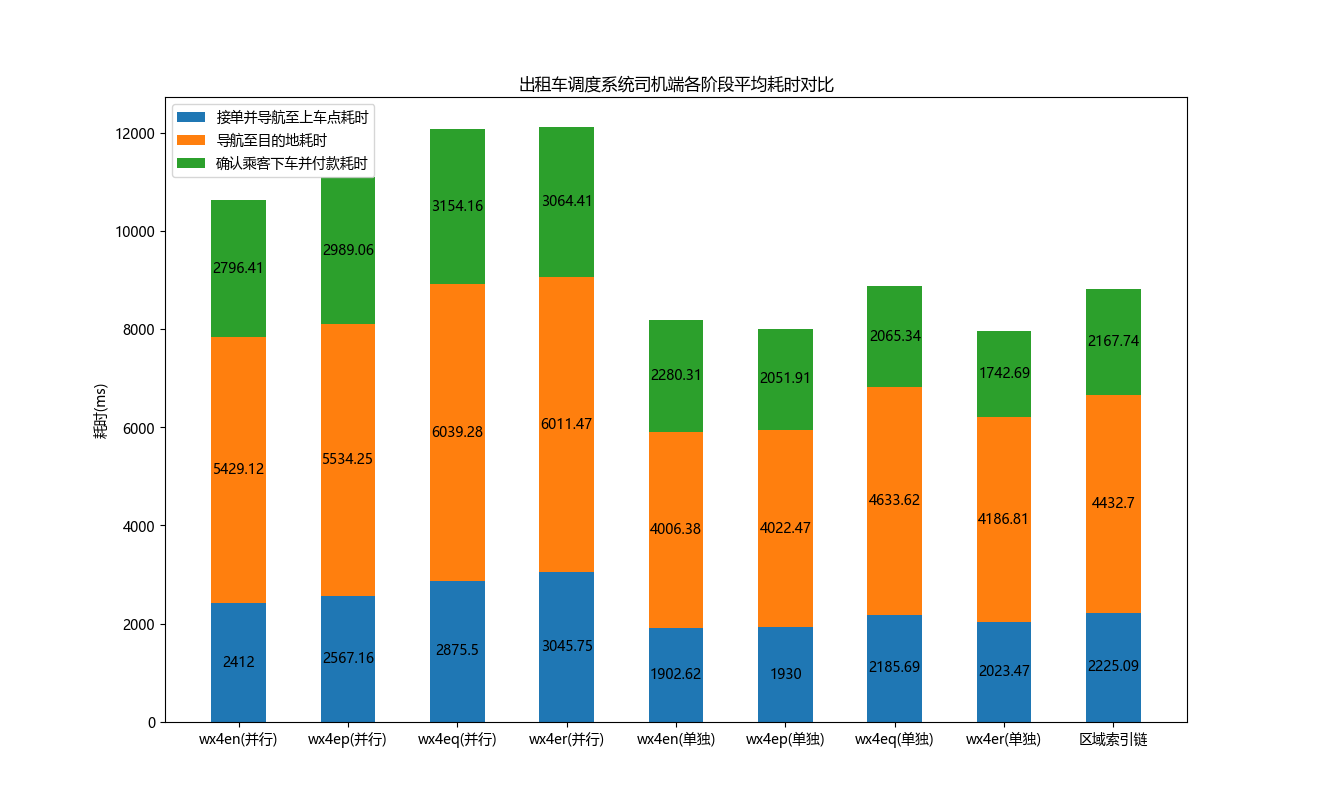
\includegraphics[width=\textwidth]{images/司机端测试.png}
    \caption{出租车调度系统司机端各阶段平均耗时对比}\label{司机端平均耗时对比} % label 用来在文中索引
\end{figure}

由图\ref{司机端模拟脚本运行逻辑}可知,司机端不存在冲突的情况(即:系统不允许同一时间有两位司机接受同一位乘客的订单),加之并行运行为测试计算机带来的较大负担,在四子链并行运行的工况下,树状区块链的性能表现大幅落后于区域索引区块链。然而,在四子链分别单独运行,测试计算机性能影响因素被减弱的工况下,树状区块链仍然以567.7毫秒的平均周转耗时优势超越了单链结构的区域索引区块链。测试证明,树状区块链相较传统区块链的性能优势并非仅来自调度系统运行时产生的诸如冲突等特殊情况,其树状结构的物理设计功不可没。然而,四条子链同时运行产生的性能开销,有可能制约树状区块链的综合性能,令区块链网络的运行效率产生不可忽视的下降。

\section{本章小结}

本章介绍了树状区块链在基于区块链的出租车调度系统上进行的各项测试及其数据分析。首先,阐述了设计测试的思路及大致方法。本章测试在采用经过分块处理的真实世界地图的基础上,采用脚本模拟司机与乘客的交互行为,在具有四个叶子链的树状区块链系统上部署出租车调度系统合约并运行模拟脚本,以收集实验数据。接下来,展示了实验环境配置,及较具体的数据准备、模拟测试的步骤方法。最后两节分别从乘客端角度和司机端角度出发,选取了不同的性能指标进行统计分析,并将结果进行可视化。针对树状区块链优于传统区块链的情况,给出了直观的展示;针对树状区块链不及传统区块链的情况,则给出了测试平台性能上限的猜想,同时设计进行补充实验加以验证该猜想,最终获得了树状区块链在实际应用场景的不同工况下的性能表现,证明了它相较传统的单链结构区块链的性能优越性。同时,证明了测试平台性能上限对树状区块链运行的影响,解释了树状区块链提供更好性能的代价之一——对系统资源的占用情况较为严重。

%%
% The BIThesis Template for Bachelor Graduation Thesis
%
% 北京理工大学毕业设计(论文)第二章节 —— 使用 XeLaTeX 编译
%
% Copyright 2020-2023 BITNP
%
% This work may be distributed and/or modified under the
% conditions of the LaTeX Project Public License, either version 1.3
% of this license or (at your option) any later version.
% The latest version of this license is in
%   http://www.latex-project.org/lppl.txt
% and version 1.3 or later is part of all distributions of LaTeX
% version 2005/12/01 or later.
%
% This work has the LPPL maintenance status `maintained'.
%
% The Current Maintainer of this work is Feng Kaiyu.
%%

\chapter{改进树状区块链——从以太坊到Substrate}

树状区块链是在以太坊官方客户端Go-Ethereum的源代码上修改而来,因此,虽然在结构上做出了很大的调整,它也继承了许多Go-Ethereum的特点,例如共识算法和EVM虚拟机等,其性能表现也依然受制于Go-Ethereum。从整体上评估,第三章的3.5.2.1节通过统计学方法,验证了以太坊顺序串行执行交易的特点,这样的执行策略使得以太坊在面对高并发请求时的处理效率不尽如人意;从局部评估,研究\cite{privateChainConsensus}表明,以太坊所使用的共识算法之一——基于工作量的证明(Proof of Work),其性能表现已落后其他更先进的算法。然而,以太坊并未在源代码层面留有太多的可扩展空间,这也意味着许多诸如更换共识算法,修改交易执行逻辑等的自定义修改在实践时困难重重,限制了在以太坊平台改良优化的空间。

Substrate\cite{substrateHome}由Parity Technologies推出,是一套开源的区块链开发框架,允许开发者针对不同的用途对链进行不同程度的定制。在Substrate诞生前,人们花费了大量的精力,试图设计一个支持多链结构的新型区块链。然而,所有这些花费的时间、金钱和精力最终导向了一个结论:当下做出的深思熟虑的选择很可能成为未来的绊脚石。这是因为随着时间的推移,区块链依赖的某些特定的技术或假设,可能会阻碍并最终扼杀创新\cite{substrateDoc}。因此,以太坊创始人之一Gavin Wood成立了Parity技术公司,力图改写这一局面。他们的处女座——以太坊客户端Parity,在相同的硬件配置环境下展现出了远胜Go-Ethereum的性能表现,提升幅度达到了可观的89.8\%\cite{parityVSgeth};在后续开发Parity自研的区块链Polkadot时,Gavin意识到,仅需将Polkadot进行抽象,剥离部分细节,即能获得一个可扩展性极强,适用范围更广的区块链框架。在2018年,Polkadot和用于开发它的区块链框架终于被分离开,成为两个独立的项目,而后者,即是本章讨论的主角——Substrate。

Substrate在设计时,严格遵循三点原则:

\begin{itemize}
    \item 将Rust编程语言作为代码库的核心编程语言。虽然Rust语言的学习曲线较为陡峭,但其极快的速度,极具辨识度的内存管理方式,灵活的抽象能力,以及可编译为WebAssembly的特点使它成为需要高性能表现,强内存安全性,及嵌入式设备友好性等特性之应用场景的不二之选;
    \item 将WebAssembly作为应用程序逻辑的执行环境。WebAssembly是一种新型代码,由万维网联盟创建,可从Rust、C、C++等语言编译获得,且受到多种JavaScript引擎的广泛支持,具有良好的兼容性\cite{wasmIntro}。Substrate的易升级性也建立于WebAssembly的基础之上:它将区块链的具体业务逻辑编译为WebAssembly字节码,并存储于区块链的数据存储区中,用户可以像发起普通交易一样发起一个申请修改链上存储的WebAssembly字节码的交易,从而便利地更新升级区块链系统;
    \item 广泛使用分层抽象、泛型实现和灵活的API作为主要的编码实践,并将库分离为不同的体系结构组件。在核心功能方面,Substrate官方提供了许多不同的实现,例如数据库层的RocksDB和ParityDB,共识层的AURA引擎和Grandpa引擎等,可以任由开发者选择;在应用功能方面,Substrate允许开发者调用官方已开发妥当的模块pallet为他们的区块链添加自定义功能,例如保存并处理账号信息的balances模块,和管理智能合约的contracts模块;不仅如此,Substrate也提供了这些模块的实现源代码,开发者可以自行下载并进行修改后引入区块链,实现功能的定制化。这一设计原则,赋予了Substrate极好的可扩展性,便于开发人员依据实际需要进行功能增删和优化改进等操作。
\end{itemize}

综合以上事实,将树状区块链自以太坊开发平台迁移至Substrate开发框架内,不仅能降低开发难度,获得更好的性能表现和安全性,还能获得更好的兼容性,令区块链能够在浏览器中乃至嵌入式设备上运行,拓宽树状区块链的应用范围。本章首先分析Substrate开发框架的节点架构,其次介绍官方提供的节点模板,演示在其上进行开发的方法,最后在节点模板的基础上,引入树状区块链的部分特性——账号地理位置,以证明将树状区块链从以太坊开发平台迁移至Substrate开发框架的可行性。

\section{Substrate节点架构}

在一个去中心化的区块链网络中,每一个节点都同时充当了客户端和服务器的作用,因为它既可以从网络中请求数据,也可以向网络提供数据。Substrate沿用了这一思想,并将其贯彻到了架构设计中。

\begin{figure}[htbp]
    \centering
    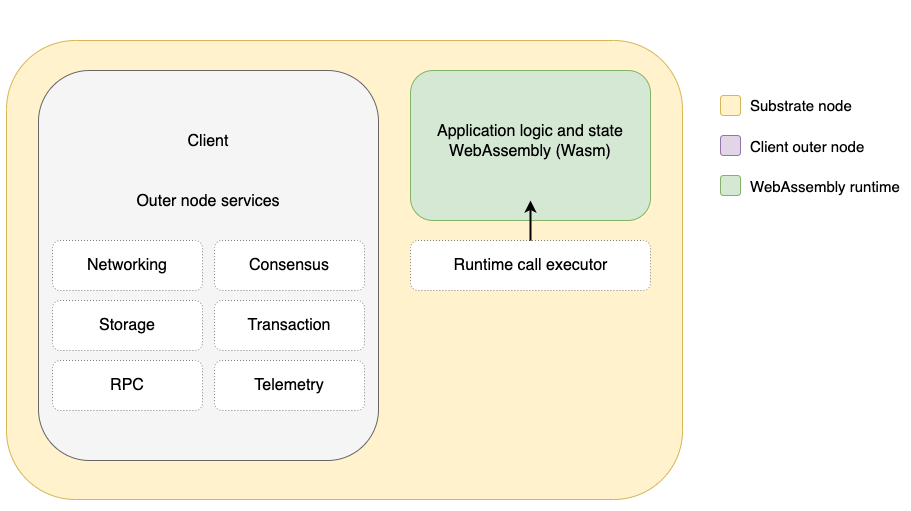
\includegraphics[width=0.8\textwidth]{images/simplified-architecture.png}
    \caption{Substrate节点架构简图}\label{Substrate节点架构简图} % label 用来在文中索引
\end{figure}

如图5-1所示,Substrate节点可以认为由两个部分组成:客户端外部节点以及WebAssembly运行时环境。

\subsection{客户端外部节点}

客户端外部节点负责运行时外部发生的活动。例如,外部节点负责发现对等节点、管理交易池、与其他节点通信以达成共识,以及响应来自外部的RPC调用或浏览器请求。

外层节点处理的一些最重要的活动包括以下几种:

\begin{itemize}
    \item 存储: 使用简单高效的键值对存储层,保存Substrate区块链不断变化的状态;
    \item 点对点网络: 使用libp2p等方式与其他的网络参与者通信;
    \item 共识: 与其他网络参与者通信,确保他们对区块链的状态达成共识;
    \item RPC API:接收入站的HTTP和WebSocket请求,以便区块链用户与网络交互;
    \item 维护节点度量: 通过内嵌的Prometheus服务器收集并提供节点度量相关的信息;
    \item 执行环境: 为运行时选择要使用的执行环境(浏览器中的WebAssembly或本地的Rust环境)然后将调用分派给所选的环境。
\end{itemize}

执行这些任务通常需要外部节点查询运行时以获取信息或向运行时提供信息。这种通信通过调用专门的runtime APIs来处理。

\subsection{WebAssembly运行时环境}

WebAssembly运行时环境确定交易是否有效,并负责处理区块链的状态转换函数的更改。因为运行时能执行它接收到的函数,所以它可以控制如何将交易包含在区块中,以及如何将区块返回到外部节点以传播或导入到其他节点。本质上,运行时负责处理区块链上发生的所有事情,它也是构建Substrate区块链节点的核心组件。

与外部节点向运行时提供信息的方式类似,运行时使用专门的host function与外部通信。

\section{Substrate节点模板介绍}

Substrate官方提供了一份开源的节点模板\footnote{https://github.com/substrate-developer-hub/substrate-node-template}。节点模板中已包含较完整的运行时环境,且允许开发者自由增删模块,实现功能定制。此外,Substrate也提供了教程文档\footnote{https://docs.substrate.io/tutorials/},辅助开发者学习使用节点模板。本节将演示在Linux环境下编译节点模板、与节点模板交互、以及为节点模板引入新模块的方法。

\subsection{环境配置}

本章的所有工作在表5-1所示的环境中进行:

\begin{table}[htbp]
    \linespread{1.5}
    \zihao{5}
    \centering
    \caption{Substrate相关工作环境}\label{Substrate相关工作环境}
    \begin{tabular}{r|l} \toprule
        中央处理器 & Intel Core i5-12500H      \\
        图形处理器 & Intel Iris Xe 80EU        \\
        内存    & 24GB                      \\
        操作系统  & Ubuntu 22.04.2 LTS        \\
        虚拟机   & VMWare Workstation Pro 17 \\
        \bottomrule
    \end{tabular}
\end{table}

同时,使用节点模板要求安装git、make、clang、curl并配置Rust开发环境\footnote{https://docs.substrate.io/install/linux/}。

使用如下指令安装包含git、make、clang、curl工具包:

\begin{lstlisting}[caption={安装工具包}, label={lst:安装工具包}]
sudo apt install build-essential
\end{lstlisting}

使用如下指令安装Rust工具链:

\begin{lstlisting}[caption={安装Rust工具链}, label={lst:安装Rust工具链}]
sudo apt install --assume-yes git clang curl libssl-dev protobuf-compiler
curl --proto '=https' --tlsv1.2 -sSf https://sh.rustup.rs | sh
source \$HOME/.cargo/env  # 刷新环境变量

rustup default stable
rustup update  # 更新rust版本为最新的稳定版

# 安装rust nightly的2023-03-21前发布的最新版
rustup update nightly-2023-03-21
rustup target add wasm32-unknown-unknown --toolchain nightly-2023-03-21
\end{lstlisting}

\subsection{使用节点模板进行开发}

本小节主要讨论编译节点模板,及使用Web UI与其交互的方法。

下载节点模板源代码后,观察\verb|runtime/Cargo.toml|。该文件记录了节点模板使用的运行时环境的各项配置。在\verb|dependencies|字段下,写有该运行时包含的各项模块名,及其版本、源代码来源等信息。关于增添新模块和修改官方提供的模块的方法,请见下一小节的介绍。

在源代码根目录中打开终端,执行\verb|cargo build --release|命令,稍事等待至编译完成后,在终端运行\verb|./target/release/node-template --dev|,即能在开发模式下启动节点模板编译而成的节点。

使用Polkadot JS APP连接到该区块链\footnote{https://polkadot.js.org/apps/?rpc=ws\%3A\%2F\%2F127.0.0.1\%3A9944\#/explorer},在页面导航栏中依次选择“账户” - “账户”,既能看到节点中预定义的账户的各项信息。在导航栏中依次选择“开发者” - “交易”,既能利用WebAssembly运行时环境中引入的模块进行各项操作。如图5-2所示,选择ALICE账户后,依次选择balances模块,选择transfer方法,在Id: AccoundId处选择FERDIE,value处填写10,随后点击“提交交易” - “签名并提交”,即可提交一个转账交易,将10单位代币从ALICE账号余额中转移到FERDIE账号余额中。

\begin{figure}[htbp]
    \centering
    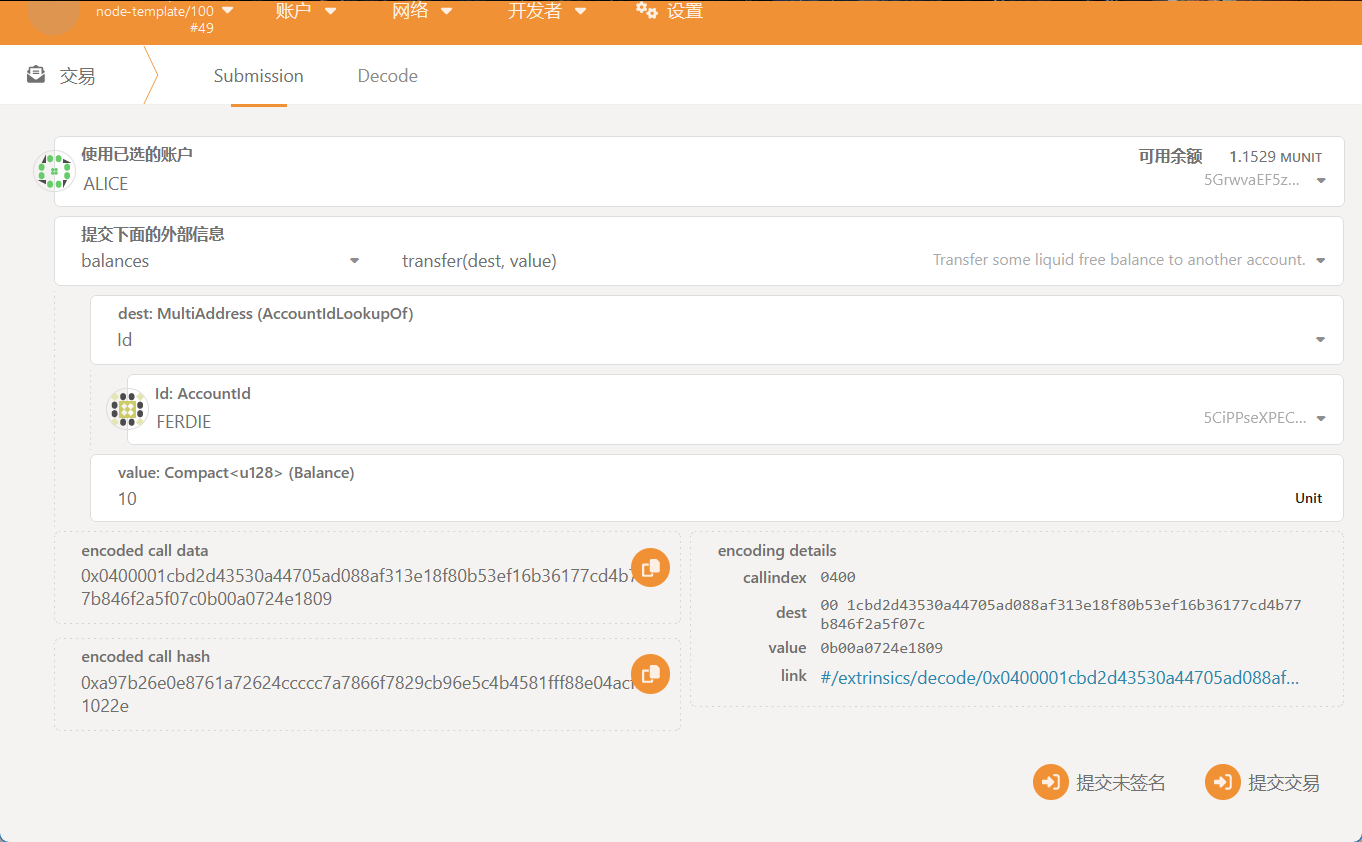
\includegraphics[width=0.8\textwidth]{images/substrateTransfer.png}
    \caption{转账交易示例}\label{转账交易示例} % label 用来在文中索引
\end{figure}

\section{为账户加入地理位置属性}

树状区块链中,为记录每个账号所处的地理位置,向账号结构中加入了地理位置这一字段,以字符串形式存储账号的Geohash编码。本小结将演示如何在Substrate节点模板上实现该效果。

\subsection{更改balances模块的引用源}

模块balances负责记录账号信息,并提供转账等与账号信息有关的功能。为实现账户信息的增添,必须对Substrate官方实现的balances模块源代码进行一定修改。

访问substrate代码仓库\footnote{https://github.com/Endericedragon/substrate/tree/polkadot-v0.9.40},切换至\verb|polkadot-0.9.40|分支以和节点模板使用的模块所处的分支一致。下载该分支的源代码并将\verb|frame/balances|目录复制到节点模板的\verb|pallets|目录中。

由于下载获得的balances模块源代码使用相对路径引用其他模块,但节点模板目录中并不存在这些路径,故需要将\verb|pallets/balances/Cargo.toml|配置文件中对其他模块的引用修改为从Github上直接引用。举例而言,对于该相对路径引用:

\begin{lstlisting}
sp-std = { version = "5.0.0", default-features = false, path = "../../primitives/std" }

\end{lstlisting}

修改为从Github上直接引用:

\begin{lstlisting}
sp-std = { version = "5.0.0", default-features = false, git = "https://github.com/paritytech/substrate.git", branch = "polkadot-v0.9.40" }
\end{lstlisting}

将所有模块的引用源更改完毕后,保存并关闭\verb|pallets/balances/Cargo.toml|,打开\verb|runtime/Cargo.toml|,将其中对模块\verb|pallet_balances|的引用从Github上引用改为从本地的\verb|pallets/balances|路径引用,修改方法与前文之所述类似,此处不再赘述。

最后,修改节点模板根目录中的\verb|Cargo.toml|:

\begin{lstlisting}
[workspace]
members = [
    "node",
    "pallets/template",
    "pallets/balances",  # <-- 新增这行
    "runtime",
]
[profile.release]
panic = "unwind"
\end{lstlisting}

保存并关闭即可。

\subsection{修改balances模块的源代码}

定义“账户”这一概念的结构体是位于pallets/balances/src/lib.rs源代码的AccountData结构体。笔者在这个结构体中,加入了一个position字段,其类型为笔者自定义的GeoHash类型。增添的代码如下:

\begin{lstlisting}[caption={为balances模块新增代码}]
const GEOHASH_LENGTH: usize = 14;

#[derive(Encode, Decode, Clone, PartialEq, Eq, RuntimeDebug, MaxEncodedLen, TypeInfo)]
pub struct Geohash([u8; GEOHASH_LENGTH]);
impl Default for Geohash {
	fn default() -> Self {
		Geohash([0; GEOHASH_LENGTH])
	}
}
impl Geohash {
	pub fn from(geohash: Vec<u8>) -> Self {
		assert!(geohash.len() <= GEOHASH_LENGTH);
		let mut position: [u8; GEOHASH_LENGTH] = [0; GEOHASH_LENGTH];
		for (i, cc) in geohash.iter().enumerate() {
			position[i] = *cc;
		}
		Geohash(position)
	}
}

// -- snip --

pub struct AccountData<Balance> {
    // --snip --

	// The position of this account, encoded in geohash
	pub position: Geohash,
}
\end{lstlisting}

每个模块均可包含一些方法,开发者可调用这些方法修改链上存储的数据,与模块交互。本小节为balances模块新增两个方法:\verb|set_position()|方法和\verb|transfer_with_position()|方法。

首先,为balances模块新增一个\verb|set_position()|方法,允许账户为自己设置地理位置:

\begin{lstlisting}
#[pallet::call]  // <-- 在pallets/balances/src/lib.rs中全局搜索这行即可找到
impl<T: Config<I>, I: 'static> Pallet<T, I> {
    // -- snip --

    // Set position for oneself
    #[pallet::call_index(6)]
    #[pallet::weight(0)]
    pub fn set_position(origin: OriginFor<T>, new_position: Vec<u8>) -> DispatchResult {
        let sender = ensure_signed(origin)?;
        Self::try_mutate_account(
            &sender,
            |target, _| {
                target.position = Geohash::from(new_position);
                Ok(())
            }
        )
    }
}
\end{lstlisting}

其次,添加一个\verb|transfer_with_position()|方法,令转账发起人提供自身位置信息,用以更新它的\verb|position|字段:

\begin{lstlisting}
#[pallet::call_index(7)]
#[pallet::weight(T::WeightInfo::transfer())]
pub fn transfer_with_position(
    origin: OriginFor<T>,
    dest: AccountIdLookupOf<T>,
    #[pallet::compact] value: T::Balance,
    position: Vec<u8>
) -> DispatchResultWithPostInfo {
    let transactor = ensure_signed(origin)?;
    let dest = T::Lookup::lookup(dest)?;
    <Self as Currency<_>>::transfer(
        &transactor,
        &dest,
        value,
        ExistenceRequirement::AllowDeath,
    )?;
    Self::try_mutate_account(
        &transactor,
        |target, _| {
            target.position = Geohash::from(position);
            Ok(().into())
        }
    )
}
\end{lstlisting}

至此,对代码的改动全部结束。以上修改已形成文档\footnote{https://github.com/Endericedragon/substrate-node-template/blob/main/修改记录.md},以便后人阅读参考。

\subsection{编译并测试修改结果}

在节点模板根目录中运行\verb|cargo build --release|命令进行编译,确认编译过程无任何错误并结束后,使用5.3节的方法启动测试链并将Web UI连接至测试链上。在导航栏上点击“开发者” - “交易”,选择ALICE账号并按图5-3所示填写交易的各项参数,以调用balances模块的\verb|set_position()|方法。提交设置位置的交易图中的wx4111b即为目标账户新地理位置的Geohash编码。需要注意的是,5.3.2小节的代码中设置了该字段的限长\verb|GEOHASH_LENGTH|为14,故提交的字符串长度必须小于该限长。

\begin{figure}[htbp]
    \centering
    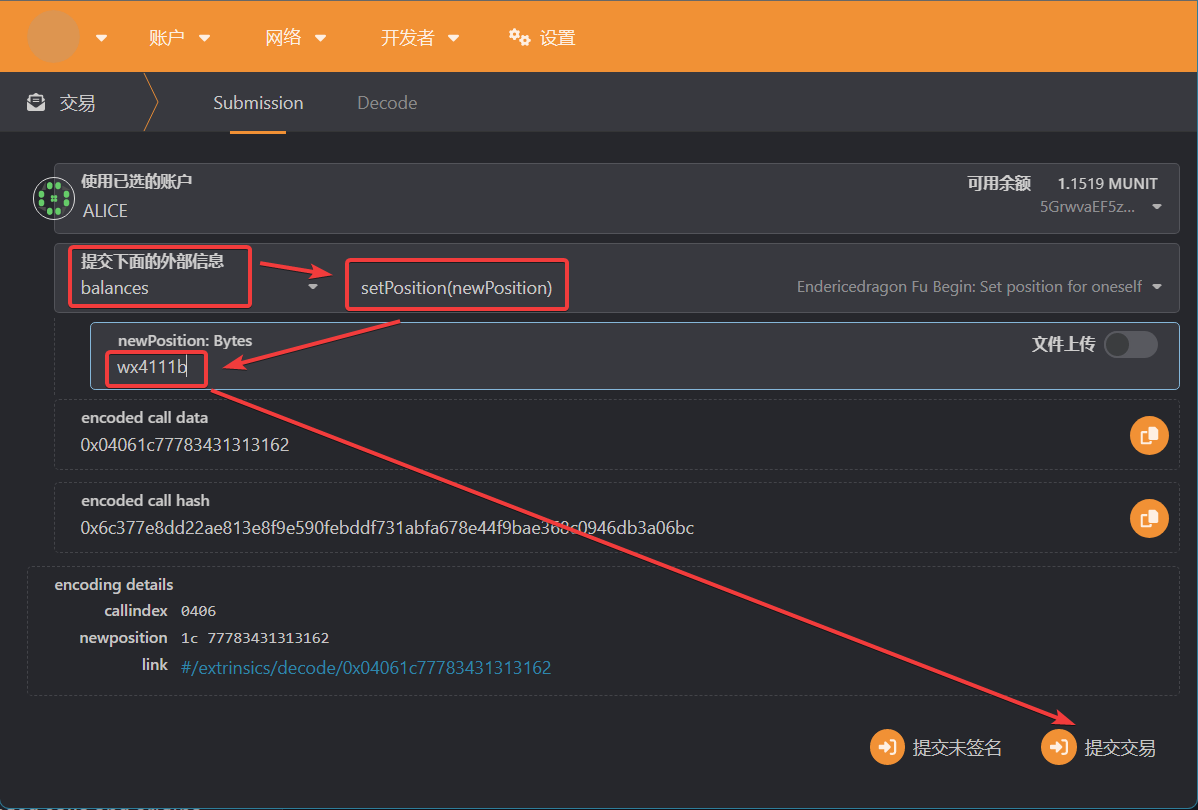
\includegraphics[width=0.8\textwidth]{images/setPos.png}
    \caption{发起设置位置交易}\label{发起设置位置交易} % label 用来在文中索引
\end{figure}

待签名并提交该交易后,点击导航栏上的“开发者” - “链状态”,按图5-4所示填写查询信息。点击界面右侧的加号,查询结果将立刻显示在界面下方,可以看到账户信息中出现了position字段,其值为0x7778343131316200000000000000。此即为提交的字符串的16进制编码,按照两位16进制编码对应一个ASCII字符的规则进行转码后,还原其记录的字符串信息即为\verb|wx4111b|,与上一步骤中提交的交易参数一致。

\begin{figure}[htbp]
    \centering
    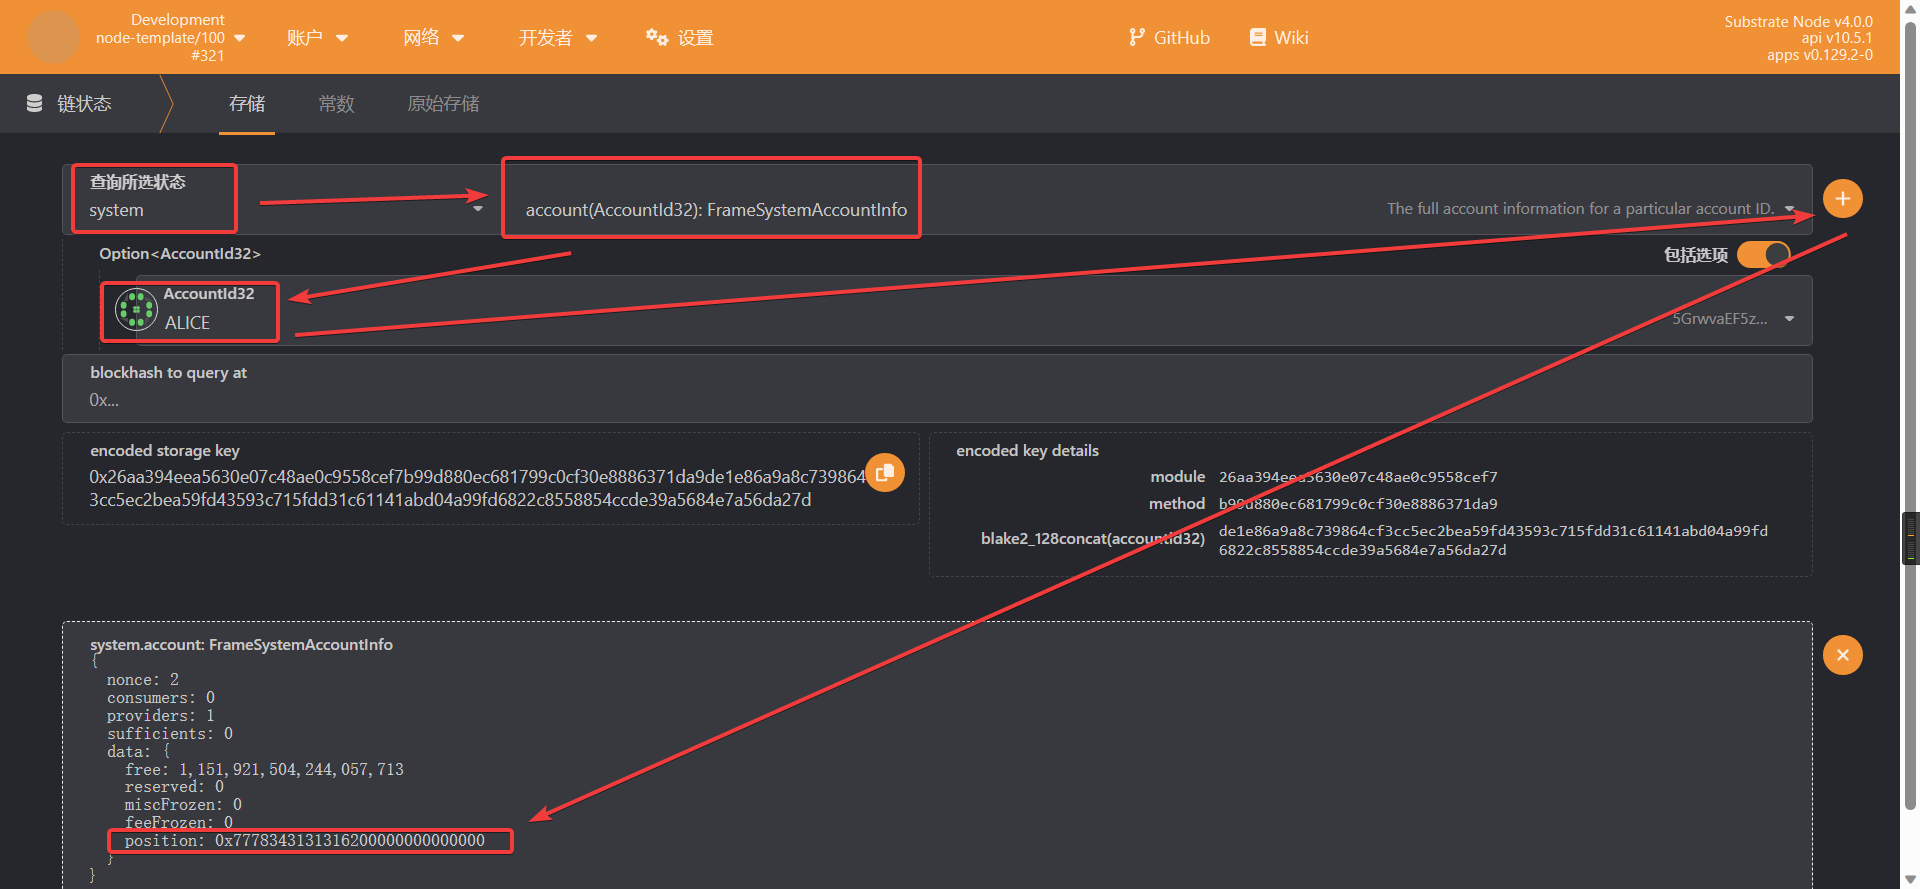
\includegraphics[width=0.8\textwidth]{images/watchAccInfo.png}
    \caption{查询账户信息}\label{查询账户信息} % label 用来在文中索引
\end{figure}

使用相似的方法,调用balances模块的\verb|transfer_with_position()|方法,令账号ALICE在wx4111c位置处发起转账,如图5-5所示。

\begin{figure}[htbp]
    \centering
    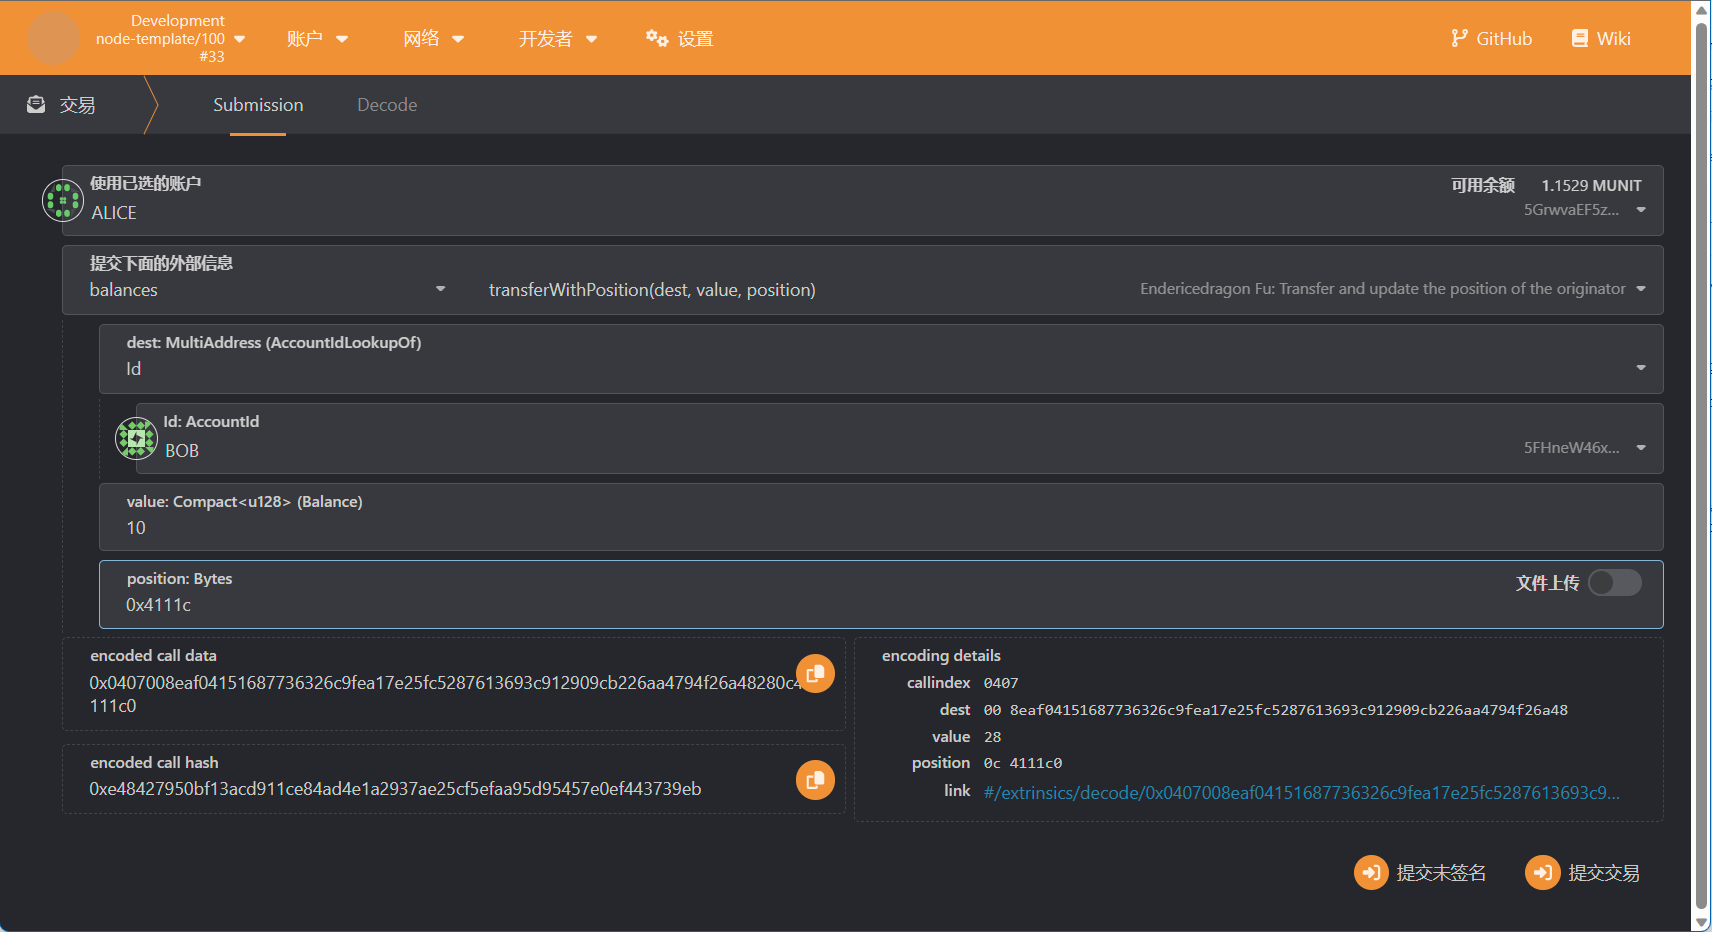
\includegraphics[width=0.8\textwidth]{images/transWithPos.png}
    \caption{调用带位置信息的转账方法}\label{调用带位置信息的转账方法} % label 用来在文中索引
\end{figure}

随后,查询转账发起人ALICE的位置信息,获得图5-6所示的输出。其中,position字段的值0x77783431313163即为ALICE的新位置Geohash编码wx4111c的16进制表示。

\begin{figure}[htbp]
    \centering
    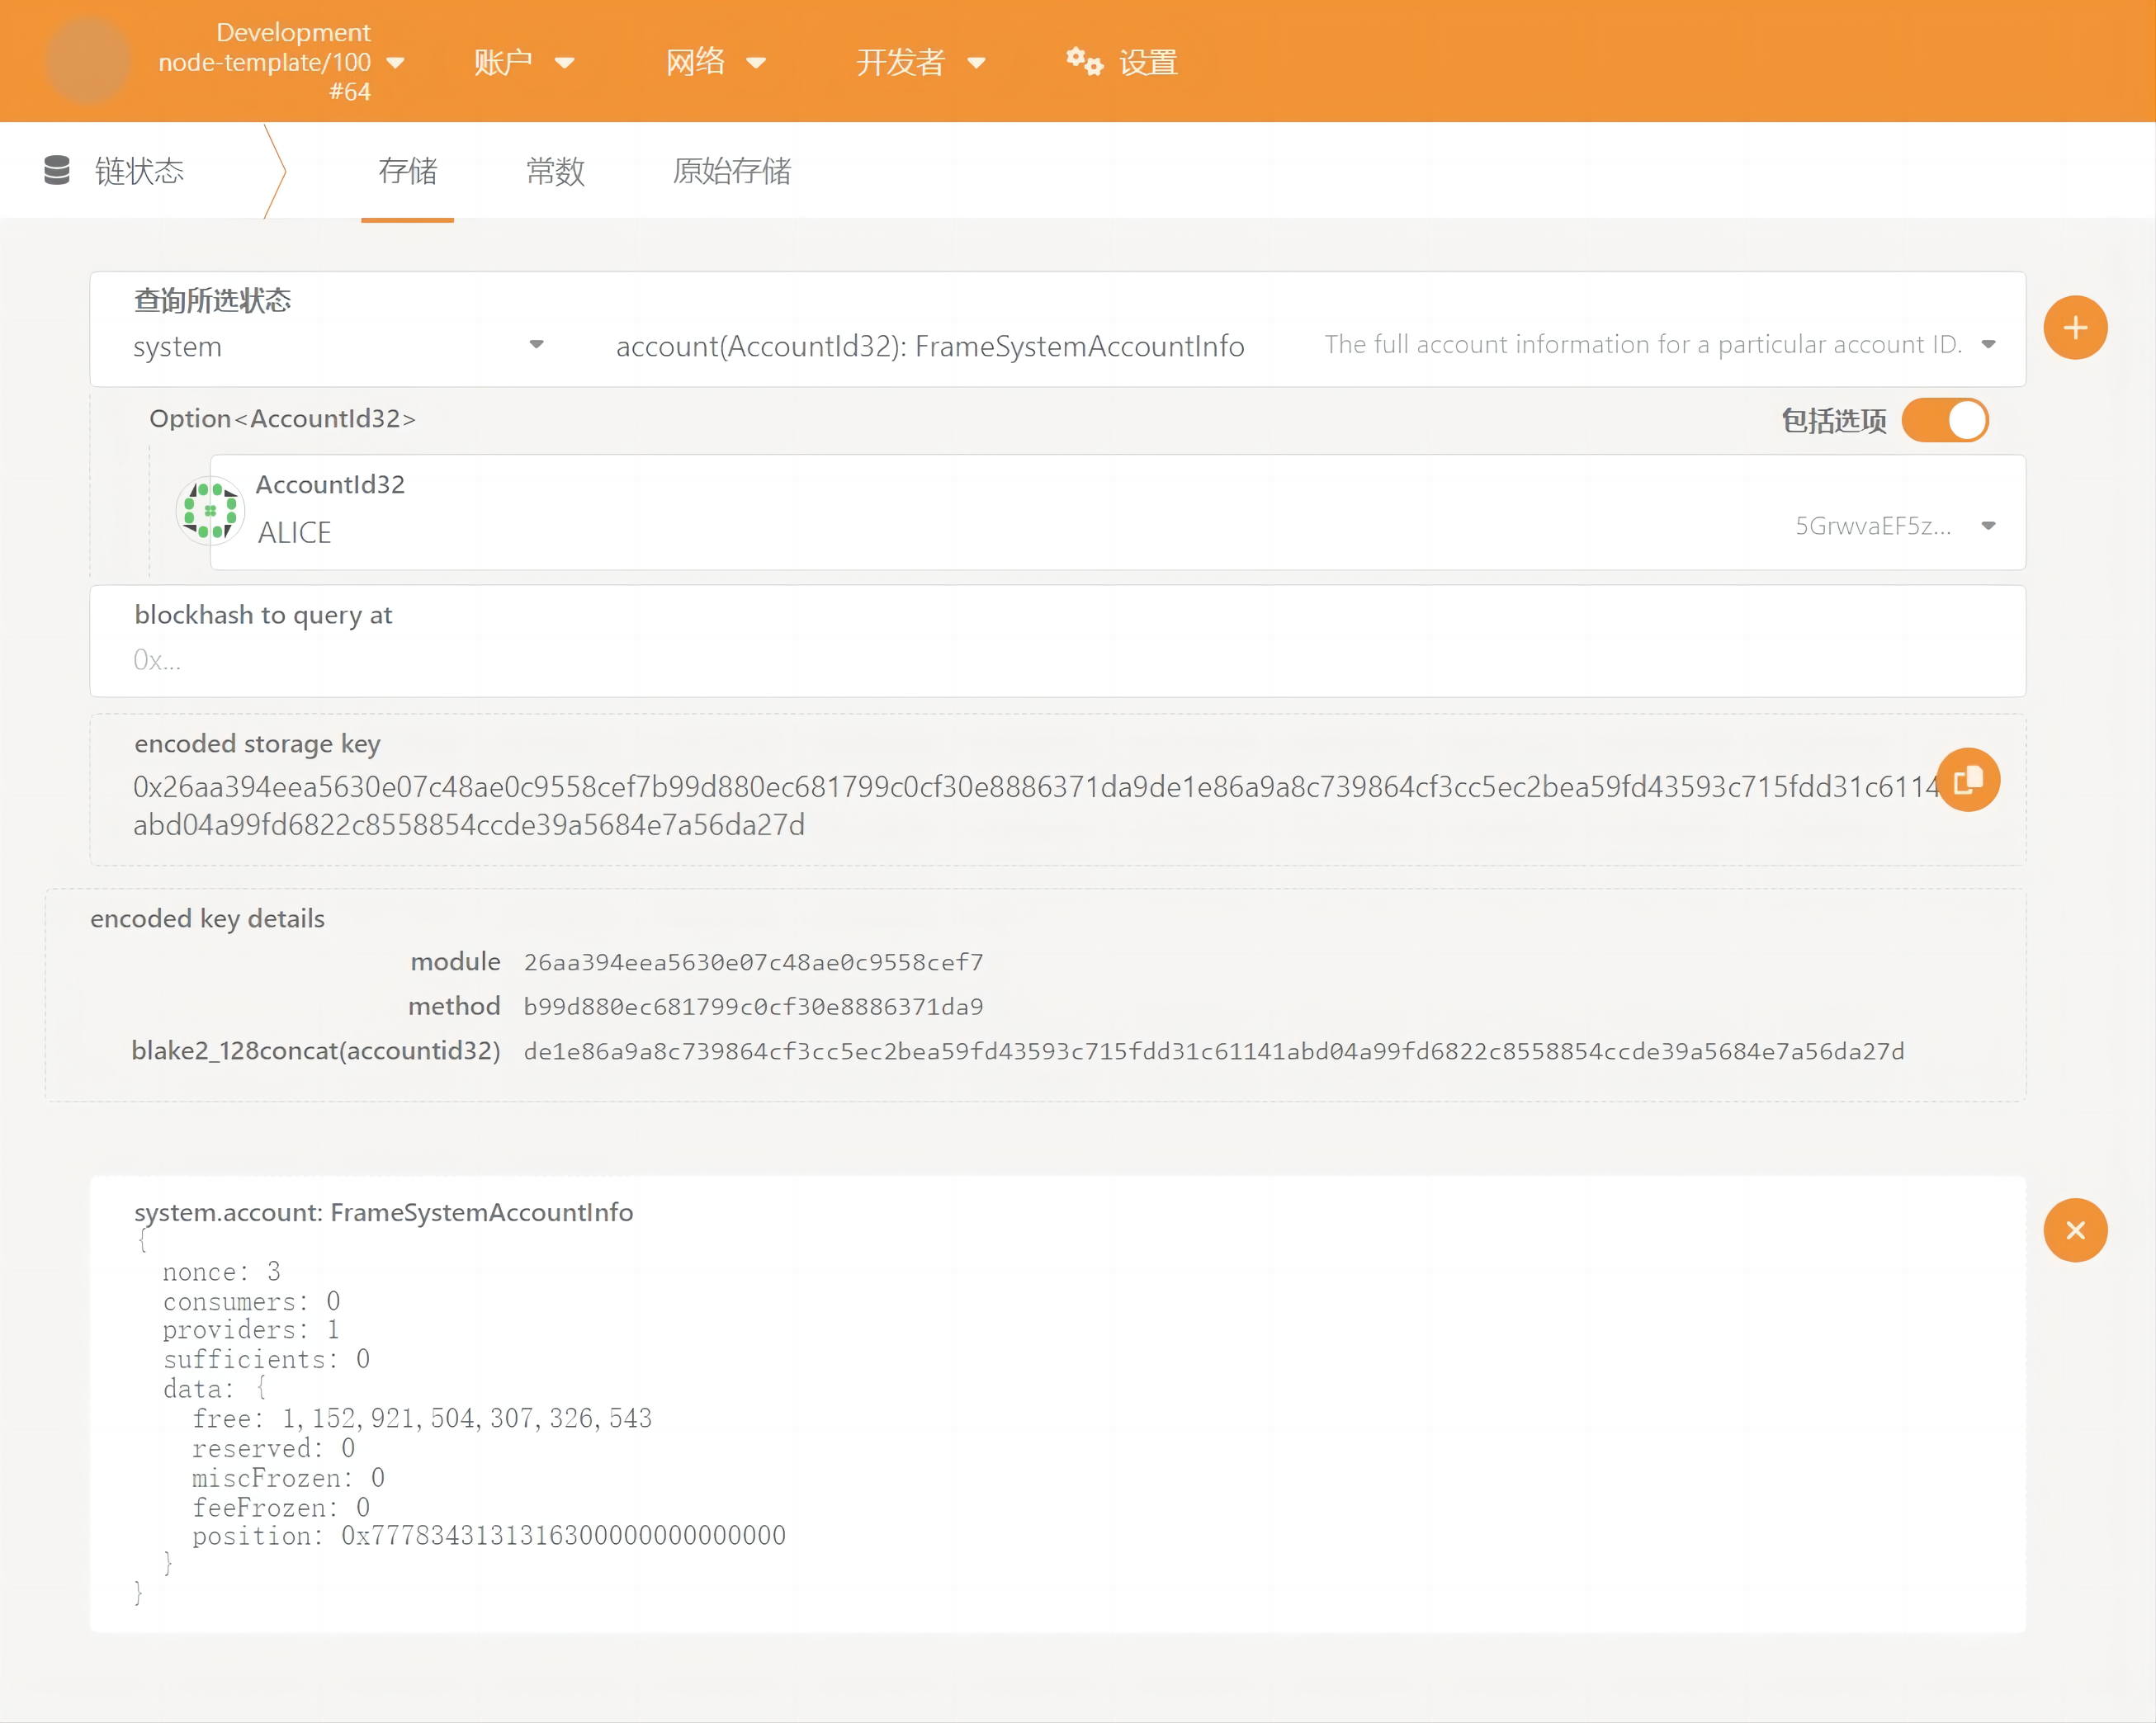
\includegraphics[width=0.8\textwidth]{images/transWithPosResult.png}
    \caption{转账发起人位置已更新}\label{转账发起人位置已更新} % label 用来在文中索引
\end{figure}

至此,账户信息中已包含地理位置字段。通过完成树状区块链部分特性在Substrate框架中的实现,本节工作证明了Substrate具有优秀的可扩展性,也为树状区块链的改进工作指明了方向。

\section{本章小结}

本章首先比较了Substrate相较以太坊的优势并介绍了Substrate的特点,阐述了树状区块链的改进思路,即将其从以太坊平台迁移至扩展性更强,综合性能更佳的Substrate开发框架。其次,介绍了Substrate的节点架构,其可分为客户端外部节点和WebAssembly运行时环境两大板块,分别负责不同类型的事务处理。最后,介绍了使用节点模板进行运行时开发的方法,并成功将树状区块链的部分功能特性迁移到节点模板上,证明了树状区块链改进思路的可行性。


% 后置部分
\backmatter

% 结论:在结论相应的 TeX 文件处进行结论部分的撰写
%%
% The BIThesis Template for Bachelor Graduation Thesis
%
% 北京理工大学毕业设计(论文)结论 —— 使用 XeLaTeX 编译
%
% Copyright 2020-2023 BITNP
%
% This work may be distributed and/or modified under the
% conditions of the LaTeX Project Public License, either version 1.3
% of this license or (at your option) any later version.
% The latest version of this license is in
%   http://www.latex-project.org/lppl.txt
% and version 1.3 or later is part of all distributions of LaTeX
% version 2005/12/01 or later.
%
% This work has the LPPL maintenance status `maintained'.
%
% The Current Maintainer of this work is Feng Kaiyu.
%
% Compile with: xelatex -> biber -> xelatex -> xelatex

\begin{conclusion}
  % 结论部分尽量不使用 \subsection 二级标题,只使用 \section 一级标题

  % 这里插入一个参考文献,仅作参考
  区块链技术以其透明性、去中心化、不可篡改等特点,在众多领域取得了瞩目的成就。然而,传统区块链的单链结构面对地理信息敏感、区块数量巨大的应用场景,无法提供令人满意的性能表现。针对该问题,实验室提出了树状区块链作为一种可行的解决办法,其采用树状结构组织多条子链,打破了单链结构的桎梏,辅之多种支持快速查询的数据结构,大大增强了区块链技术在上述几种应用场景中的适用性。

  本文以基于区块链的出租车调度系统作为应用背景,针对树状区块链进行了相关调研、测试与部分重写工作。

  % 首先,在树状区块链的前身——区域索引区块链上,复现了出租车调度系统相关工作,证明了该系统的可用性,同时指出并修复了实验室原有工作的疏漏,最后将以上工作归纳为详尽的手册,为树状区块链上运行出租车调度系统的测试奠定了基础。
  首先,在树状区块链的前身——区域索引区块链上,复现了出租车调度系统相关工作,证明了该系统的可用性,奠定了以出租车调度系统为背景的树状区块链测试的基础。

  其次,本文介绍了树状区块链的跨子链转账功能,详细解释了该功能的作用和代价,接着设计了数套测试,考察了树状区块链执行跨子链转账功能在不同负载情况下的执行效率,最后对测试结果进行分析,并建立简单的数学模型,供开发者在不同场景下选择不同区块链实现参考。

  在上述工作基础上,本文设计并进行了基于区块链的出租车调度系统在不同结构区块链上运行的对比测试,在收集测试数据后,以乘客端视角和司机端视角,对测试数据进行处理、汇总和可视化,针对树状区块链和区域索引区块链的长处短板进行分析,最后完成了补充实验的设计及进行,证明分析得出的猜想。

  最后,本文介绍了使用Rust重写树状区块链的合理性,并移植了部分树状区块链的特性到基于Rust实现的区块链框架——Substrate中,证明了该重写方案的可行性。通过对比Substrate区块链开发框架与以太坊开发平台的优势和不足,笔者强调了继续在以太坊上进行树状区块链开发的局限性,阐明了使用Rust重写树状区块链这一迁移方案的合理性。随后,本文对树状区块链当前在Golang上的实现进行了分析,评估了完成该重写工作的大致工作量;为证明该移植方案的确实存在可行性,本文选择了账户地理位置信息这一树状区块链特性,添加到Substrate的官方节点模板中,并成功进行了验证性演示。

虽然本文基本完成了有关树状区块链的系统性测试,提出了使用Rust编程语言重写树状区块链的可行方案并进行了部分验证,但笔者认为该项目仍有可拓展的研究内容,例如:

\begin{itemize}
  \item 第三章中,基于测试结果建立的模型较为简单;在进行动态查询复杂度分析时,仅考察了深度为2的树状区块链网络。若能针对更复杂的网络拓扑结进行分析,构建的数学模型将更能贴近树状区块链在实际场景中的工作情况;
  \item 第四章中,四条子链并行运行所获得的结果并不理想。虽然笔者提出了测试计算机的性能上限影响了树状区块链的性能发挥的猜想,并设计补充实验加以验证,但若能在性能更好的测试平台上进行该实验,获得的数据才能更有力地证明这一猜想;
  \item 第五章中,已针对账户地理位置信息完成了一部分树状区块链的特性移植。可以继续进行特性移植,将树状区块链的所有功能特性使用Substrate平台重写,完善该项工作。
\end{itemize}

  % TODO: 对未来的展望
\end{conclusion}

% 参考文献:如无特殊需要,参考文献相应的 TeX 文件无需改动,添加参考文献请使用 BibTeX 的格式
%   添加至 misc/ref.bib 中,并在正文的相应位置使用 \cite{xxx} 的格式引用参考文献
%%
% The BIThesis Template for Bachelor Graduation Thesis
%
% 北京理工大学毕业设计(论文)参考文献 —— 使用 XeLaTeX 编译
%
% Copyright 2020-2023 BITNP
%
% This work may be distributed and/or modified under the
% conditions of the LaTeX Project Public License, either version 1.3
% of this license or (at your option) any later version.
% The latest version of this license is in
%   http://www.latex-project.org/lppl.txt
% and version 1.3 or later is part of all distributions of LaTeX
% version 2005/12/01 or later.
%
% This work has the LPPL maintenance status `maintained'.
%
% The Current Maintainer of this work is Feng Kaiyu.
%
% Compile with: xelatex -> biber -> xelatex -> xelatex
%
% 如无特殊需要,本页面无需更改

\begin{bibprint}

% -------------------------------- 示例内容(正式使用时请删除) ------------------------------------- %

% 抑制多次调用 \printbibliography 的 warning,只有示例代码会需要此语句。
% \BiblatexSplitbibDefernumbersWarningOff

% \textcolor{blue}{参考文献书写规范}

% \textcolor{blue}{参考国家标准《信息与文献参考文献著录规则》【GB/T 7714—2015】,参考文献书写规范如下:}

% \textcolor{blue}{\textbf{1. 文献类型和标识代码}}

% \textcolor{blue}{普通图书:M}\qquad\textcolor{blue}{会议录:C}\qquad\textcolor{blue}{汇编:G}\qquad\textcolor{blue}{报纸:N}

% \textcolor{blue}{期刊:J}\qquad\textcolor{blue}{学位论文:D}\qquad\textcolor{blue}{报告:R}\qquad\textcolor{blue}{标准:S}

% \textcolor{blue}{专利:P}\qquad\textcolor{blue}{数据库:DB}\qquad\textcolor{blue}{计算机程序:CP}\qquad\textcolor{blue}{电子公告:EB}

% \textcolor{blue}{档案:A}\qquad\textcolor{blue}{舆图:CM}\qquad\textcolor{blue}{数据集:DS}\qquad\textcolor{blue}{其他:Z}

% \textcolor{blue}{\textbf{2. 不同类别文献书写规范要求}}

% \textcolor{blue}{\textbf{期刊}}

% \noindent\textcolor{blue}{[序号]主要责任者. 文献题名[J]. 刊名, 出版年份, 卷号(期号): 起止页码. }



% \textcolor{blue}{\textbf{普通图书}}

% \noindent\textcolor{blue}{[序号]主要责任者. 文献题名[M]. 出版地: 出版者, 出版年. 起止页码. }

% \textcolor{blue}{\textbf{会议论文集}}

% \noindent\textcolor{blue}{[序号]析出责任者. 析出题名[A]. 见(英文用In): 主编. 论文集名[C]. (供选择项: 会议名, 会址, 开会年)出版地: 出版者, 出版年. 起止页码. }

% \textcolor{blue}{\textbf{专著中析出的文献}}

% \noindent\textcolor{blue}{[序号]析出责任者. 析出题名[A]. 见(英文用In): 专著责任者. 书名[M]. 出版地: 出版者, 出版年.起止页码. }

% \textcolor{blue}{\textbf{学位论文}}

% \noindent\textcolor{blue}{[序号]主要责任者. 文献题名[D]. 保存地: 保存单位, 年份. }

% \textcolor{blue}{\textbf{报告}}

% \noindent\textcolor{blue}{[序号]主要责任者. 文献题名[R]. 报告地: 报告会主办单位, 年份. }

% \textcolor{blue}{\textbf{专利文献}}

% \noindent\textcolor{blue}{[序号]专利所有者. 专利题名[P]. 专利国别: 专利号, 发布日期. }

% \textcolor{blue}{\textbf{国际、国家标准}}

% \noindent\textcolor{blue}{[序号]标准代号. 标准名称[S]. 出版地: 出版者, 出版年. }

% \textcolor{blue}{\textbf{报纸文章}}

% \noindent\textcolor{blue}{[序号]主要责任者. 文献题名[N]. 报纸名, 出版年, 月(日): 版次. }

% \textcolor{blue}{\textbf{电子文献}}

% \noindent\textcolor{blue}{[序号]主要责任者. 电子文献题名[文献类型/载体类型]. 电子文献的出版或可获得地址(电子文献地址用文字表述), 发表或更新日期/引用日期(任选). }
% \cite{yaoboyuan}

% \textcolor{blue}{关于参考文献的未尽事项可参考国家标准《信息与文献参考文献著录规则》(GB/T 7714—2015)}

% \printbibliography [type=article,heading=none]
% \printbibliography [keyword={book},heading=none]
% \printbibliography [type=inproceedings,heading=none]
% \printbibliography [type=inbook,heading=none]
% \printbibliography [keyword={thesis},heading=none]
% \printbibliography [keyword={techreport},heading=none]
% \printbibliography [type=patent,heading=none]
% \printbibliography [keyword={standard},heading=none]
% \printbibliography [keyword={newspaper},heading=none]
% \printbibliography [keyword={online},heading=none]

% 在使用时,请删除/注释上方示例内容,并启用下方语句以输出所有的参考文献
\printbibliography[heading=none]
\end{bibprint}

% 附录:在附录相应的 TeX 文件处进行附录部分的撰写
%%
% The BIThesis Template for Bachelor Graduation Thesis
%
% 北京理工大学毕业设计(论文)附录 —— 使用 XeLaTeX 编译
%
% Copyright 2020-2023 BITNP
%
% This work may be distributed and/or modified under the
% conditions of the LaTeX Project Public License, either version 1.3
% of this license or (at your option) any later version.
% The latest version of this license is in
%   http://www.latex-project.org/lppl.txt
% and version 1.3 or later is part of all distributions of LaTeX
% version 2005/12/01 or later.
%
% This work has the LPPL maintenance status `maintained'.
%
% The Current Maintainer of this work is Feng Kaiyu.
%
% Compile with: xelatex -> biber -> xelatex -> xelatex

\begin{appendices}
  % 这里示范一下添加多个附录的方法:
  % 使用 \section 来添加一个附录

  \section{创世配置文件}

  \begin{lstlisting}[caption={创世配置文件}, label={lst:创世配置文件}]
    {
        "config": {
            "chainId": 666,
            "homesteadBlock": 0,
            "eip150Block": 0,
            "eip150Hash": "0x0000000000000000000000000000000000000000000000000000000000000000",
            "eip155Block": 0,
            "eip158Block": 0,
            "byzantiumBlock": 0,
            "constantinopleBlock": 0,
            "petersburgBlock": 0,
            "istanbulBlock": 0,
            "ethash": {}
        },
        "nonce": "0x0",
        "timestamp": "0x5ddf8f3e",
        "extraData": "0x0000000000000000000000000000000000000000000000000000000000000000",
        "gasLimit": "0xffffffff",
        "difficulty": "0x20000",
        "mixHash": "0x0000000000000000000000000000000000000000000000000000000000000000",
        "coinbase": "0x0000000000000000000000000000000000000000",
        "alloc": {},
        "number": "0x0",
        "gasUsed": "0x0",
        "parentHash": "0x0000000000000000000000000000000000000000000000000000000000000000"
    }
  \end{lstlisting}

  一些关键字段的解释如下:

  \begin{itemize}
    \item gasLimit:区块链为防止恶意参与者不停发送交易耗尽服务器资源,往往都对交易进行“收费”。gasLimit字段限制一次交易的最大花费。为保证实验成功,故此处设置得较大。
    \item difficulty:挖矿难度。难度越低,越容易挖到符合要求的新区块,出块速度也越高。
    \item alloc:记录链上部分账户的余额等信息。由于该创世配置文件乃是为尚未准备账户的全新区块链所准备,故此项为一个空白的JavaScript对象。
  \end{itemize}

  \section{合约部署的代码模板}

  \begin{lstlisting}[caption={合约部署代码模板}, label={lst:合约部署代码模板}]
    abi = JSON.parse("经过压缩转义后的ABI")
    bytecode = "获得的字节码字符串"

    Contract = web3.eth.contract(abi);
    web3.eth.estimateGas({data: bytecode})
    contractInstance = Contract.new({
        from: web3.eth.accounts[0],
        data: bytecode,
        gas: '3000000',
        position:"w2511111111111",
        txtime:277001
      },function (e, contract){
        console.log(e, contract);
        if(!e){
            if(!contract.address) {
                console.log("Contract transaction send: TransactionHash: " + contract.transactionHash + " waiting to be mined...");
            } else {
                console.log("Contract mined! Address: " + contract.address);
                console.log(contract);
            }
        }
    });
\end{lstlisting}

  \section{跨链转账测试的数据可视化代码}
  \begin{lstlisting}[caption={跨链转账测试的数据可视化}, label={lst:跨链转账测试的数据可视化}]
    import matplotlib.pyplot as plt
    from matplotlib.axes._axes import Axes
    from matplotlib.figure import Figure
    import numpy as np

    plt.style.use('_mpl-gallery')

    # make data
    times: list[int] = [1683465655]
    with open("tx_result_w11.txt", "r", encoding="utf-8") as f:
        times += [int(each.split('\t')[1]) for each in f.readlines()]

    times.sort()

    x = range(len(times) - 1)
    y = [times[i] - times[i - 1] for i in range(1, len(times))]

    # plot
    fig, ax = plt.subplots()
    fig: Figure
    ax: Axes

    stem = ax.stem(x, y)

    # ax.set(
    #     xlim=(0, 8), xticks=np.arange(1, 8),
    #     ylim=(0, 8), yticks=np.arange(1, 8)
    # )

    for (i, j) in zip(x, y):
        plt.text(i, j + 0.3, j)

    # ax.bar_label(stem)

    plt.show()
  \end{lstlisting}
\end{appendices}

% 致谢:在致谢相应的 TeX 文件处进行致谢部分的撰写
%%
% The BIThesis Template for Bachelor Graduation Thesis
%
% 北京理工大学毕业设计(论文)致谢 —— 使用 XeLaTeX 编译
%
% Copyright 2020-2023 BITNP
%
% This work may be distributed and/or modified under the
% conditions of the LaTeX Project Public License, either version 1.3
% of this license or (at your option) any later version.
% The latest version of this license is in
%   http://www.latex-project.org/lppl.txt
% and version 1.3 or later is part of all distributions of LaTeX
% version 2005/12/01 or later.
%
% This work has the LPPL maintenance status `maintained'.
%
% The Current Maintainer of this work is Feng Kaiyu.
%
% Compile with: xelatex -> biber -> xelatex -> xelatex

% 致谢部分尽量不使用 \subsection 二级标题,只使用 \section 一级标题
\begin{acknowledgements}
  我曾幻想,当我完成毕业设计,心中会作如何感想呢?是完成一项挑战的成就感?抑或是将知识应用于实践的喜悦?然而,放下执笔之手,心中却只有了却一桩大事的释然。回想那遥远的秋天,怀揣好奇与些许不安踏入北京理工大学的校门,拘谨地与未来四年的同窗们打招呼的情形仿佛就在昨日一般。一路走来,虽有新冠疫情侵扰、求学之路上亦非一帆风顺,但我十分庆幸高三并非我知识储备与智力的巅峰。四年求学之路,终有所收获。

  我想感谢我的导师陆慧梅老师以及向勇老师。在我迷茫低落之际,陆老师总能以淳淳教诲重新唤起我的信心,坚定我的目标,令我能够走出迷雾,继续前行。在课题方向选择、研究思路方面,向老师给了我相当的支持,并以严格而非严苛的要求因材施教,敦促我在个人能力范围内保质保量地完成毕业设计。

  我想感谢实验室的成佳壮学长、万琦玲学姐、周畅学姐。在有关出租车调度系统和树状区块链的使用、测试、调试等过程中,他们提供了宝贵的帮助。万学姐的复现手册、成学长和周学姐组织的线上研讨会,无不令我在研究课题的过程中减少一份疑惑,增添一份信心。

  感谢我的父母傅盛阳先生和赵晓斐女士,他们在我最迷茫的低谷期毅然决然地选择无条件的理解和包容,为我出谋划策,安定我心。我的毕设能完成至如此程度,离不开他们的大力支持。

  感谢所有老师,和与我一同度过四年美好时光的同学们。有了他们,我的求学之路上,就有了朗朗书声,欢歌笑语相伴。
\end{acknowledgements}


\end{document}
